% !TeX root = ../dd.tex

\section{Architectural Design}\label{ch:2}

\subsection{Overview}
% High-level component and their interaction
To ensure high maintainability, scalability and security, the service is structured according to the well-established three-tier architecture.
Figure \ref{fig:overview-architecture} shows how the tiers are divided, and what are the relations between key components of the system.

\begin{figure}[H]
    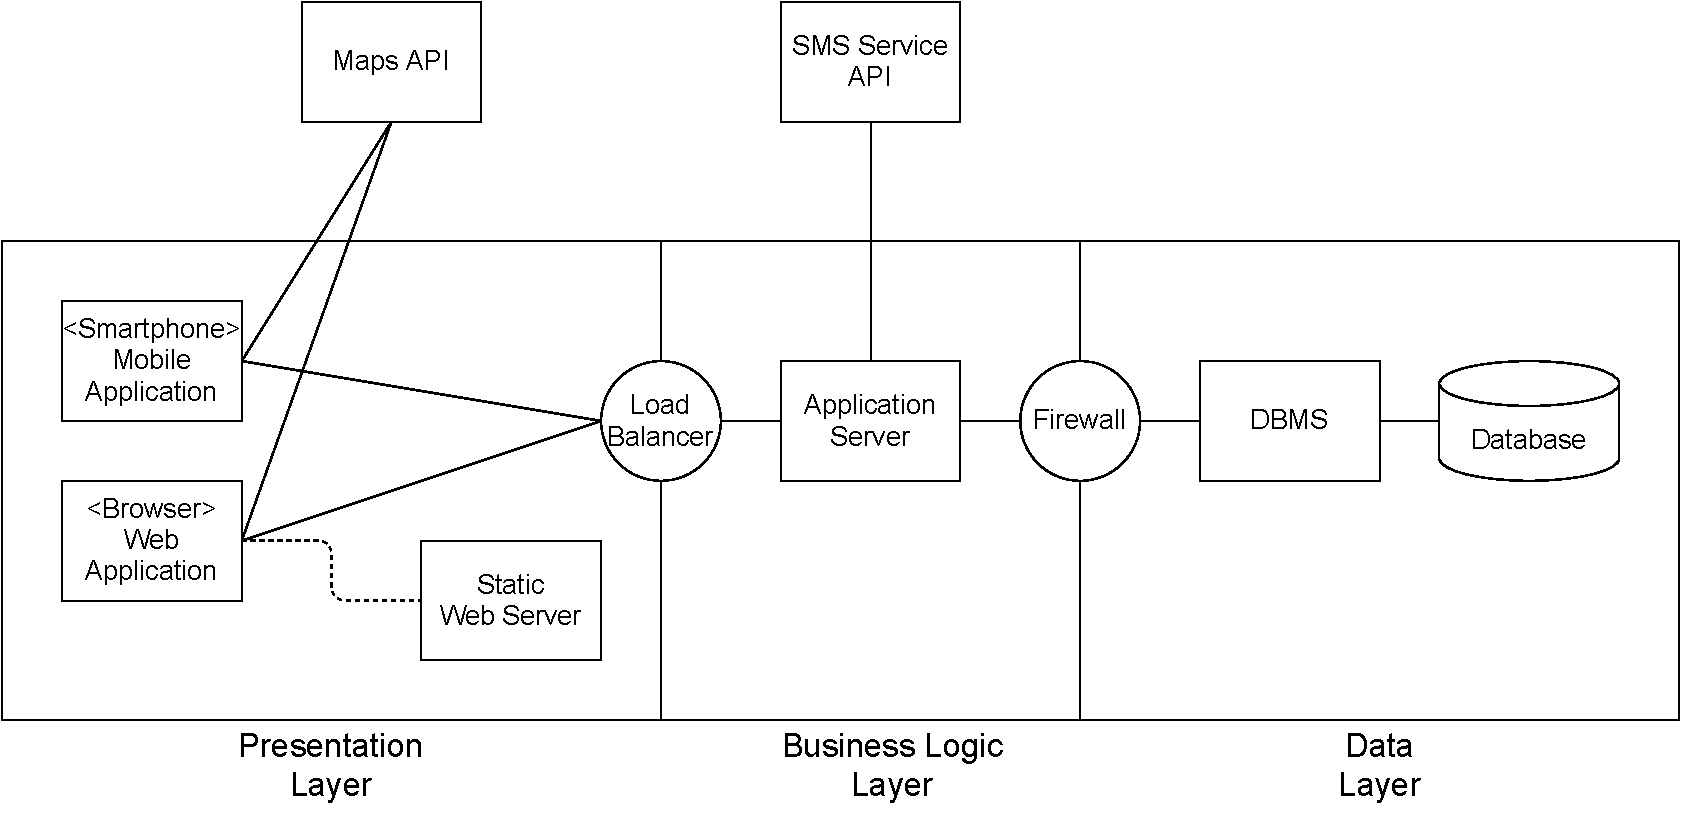
\includegraphics[width=\linewidth]{images/draw.io/overview_architecture.pdf}
    \caption{Overall architecture of the System}
    \label{fig:overview-architecture}
\end{figure}

The main components are the following:

\begin{itemize}
    \item \textbf{Mobile Application} The application is installed on the user's device through its store platform service. The application allows the user to interact with the service and receive notifications from the server.
    \item \textbf{Web Application} The web application allows users to access the same services available on the mobile app through any device, but it's not guaranteed that it can receive notifications. In addition to that, store managers may access a dedicated panel to configure additional parameters.
    \item \textbf{Static Web Server} It serves the client's browser a bundle that contains the web application code (compressed HTML and JavaScript). It has no ties with the application server.
    \item \textbf{Application Server} It's the main backend component of the service, and contains the logic to process requests made against its API from the clients.
    \item \textbf{Database} It's the component that manages the connection to the database.
    \item \textbf{External Services} These services provides functionalities that the service can't provide by itself without additional infrastructure. They incluse a \emph{SMS Service} to send messages to users, a \emph{Maps API} to visualize the location of the store on the user's device, and a \emph{Notification API} to send push notifications to users.
\end{itemize}

\subsection{Component View}
\begin{figure}[H]
    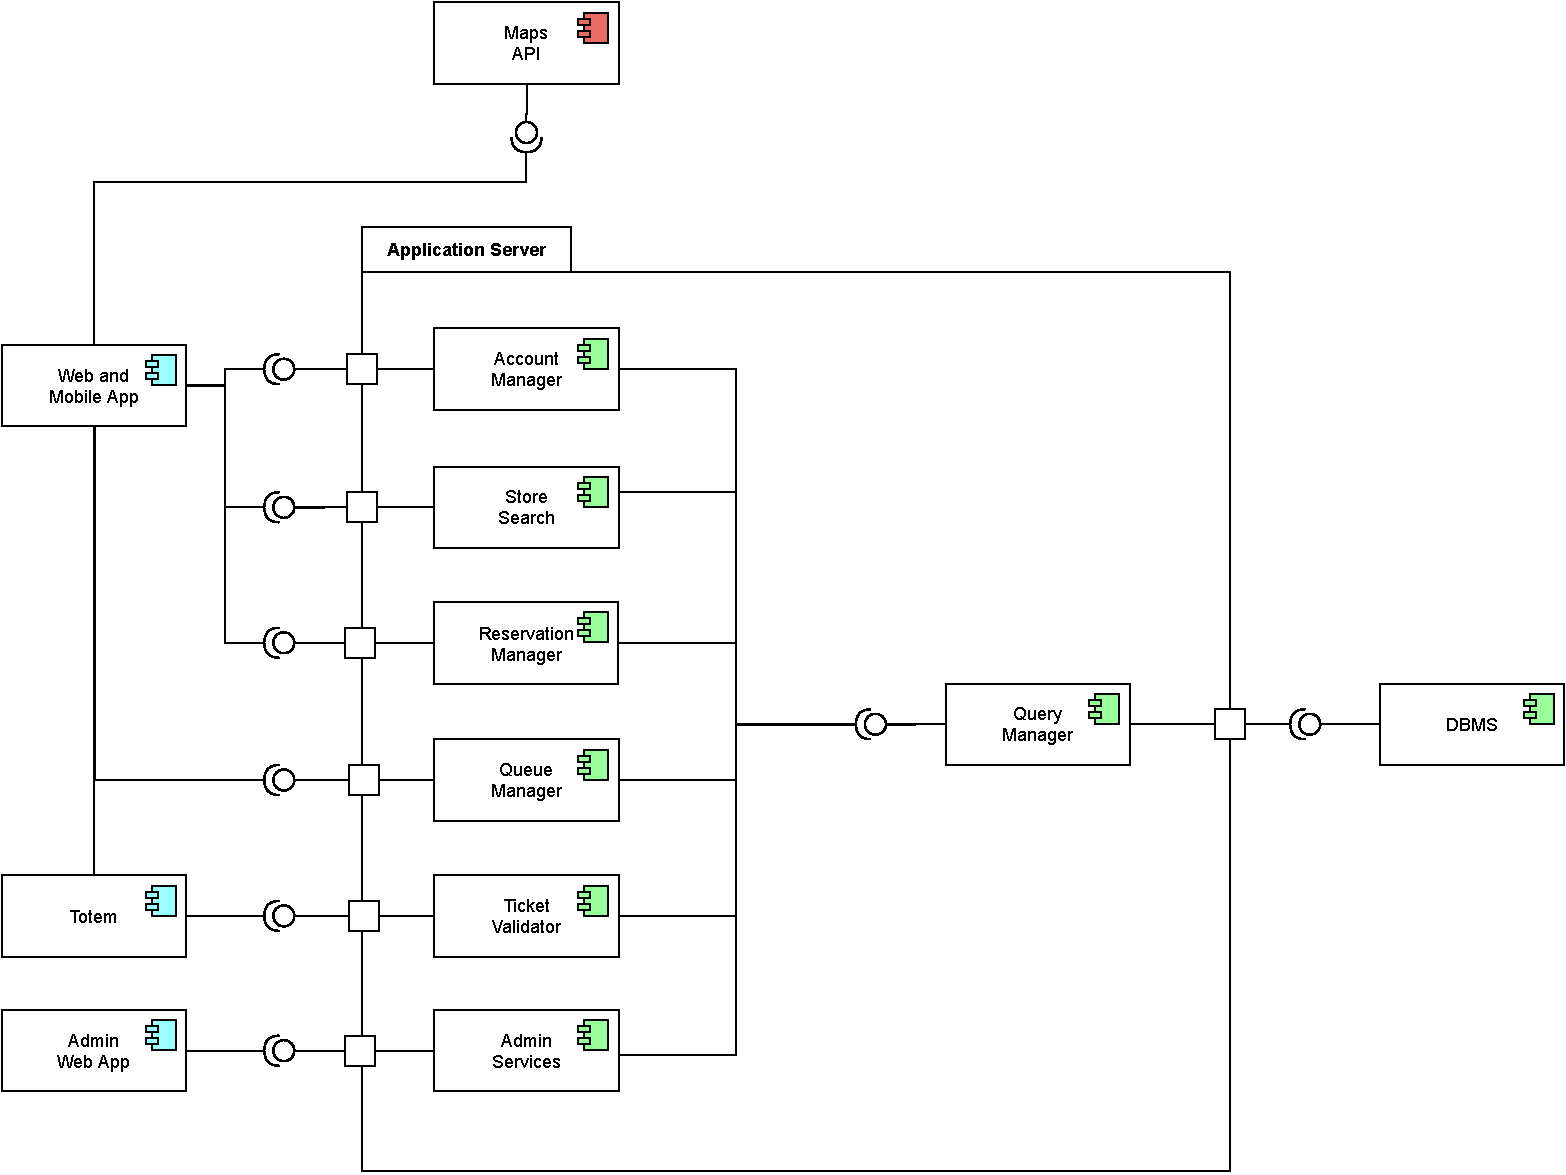
\includegraphics[width=\linewidth]{images/draw.io/component.pdf}
    \caption{Global Component Diagram of the System}
    \label{fig:component}
\end{figure}

\subsubsection{Client Components}
The client components make up the entire frontend logic of the system.
The role of the client components is to interface the user with the application server API, rendering interfaces and requesting data upon requests. As the entire UI is encoded in the client components, only a minimum amount of data will be passed between frontend and backend, reducing useless and repetitive traffic.
The client components are divided in three main subcomponents, each targeted at a different type of user:
\begin{itemize}
    \item \textbf{Web and Mobile App} are targeted at the user. They contain all the logic required to request and display information about stores, reservation, and queues. They are united in a single component as they will share most of the code and will use the same API.
    \item \textbf{Totem} will be deployed in the totems inside the store. They require a more limited set of functionalities compared to the user components (namely, the possibility of joining the queue). Additionally, it will send request to the Application Server in order to validate tickets, and provides hardware interfaces in order to interact with physical devices like doors or turnstiles. On the UX side, it will contain the functionality needed to print tickets and to display the current status of the queue.
    \item \textbf{Admin Web App} is intended for internal use only. It is the platform through which the store managers will add, remove and manage the stores. It will connect to a different API in order to separate the functionalities and the responsibilities as much as possible.
\end{itemize}


\subsubsection{Application Server Components}
The Application Server Components contain all the business logic needed to provide the functionalities of the application, communicating with the DBMS when needed and responding to queries sent by the Client Components.
The Application Server Components are:

\paragraph{Query Manager} is a component that handles the interactions with the DBMS, acting as a mediator between the business and data layer. It sends to and retrieves data from the database exposing a limited and higher level set of functionalities compared to a database query language.

\paragraph{Account Manager} handles everything related to user accounts. In particular it will offer functionalities related to creating new accounts, logging in, and setting preferences and notifications. When creating an account it will communicate with an external \textbf{SMS API} in order to send confirmation codes.

\paragraph{Store Search} allows users to search stores at specific locations and with the aid of filters. It doesn't require an external API.

\paragraph{Store Handler} is a top-level component that includes four sub-compontent to better modularize the functionalities it provides.
Its purpose is to manage the interactions between customers and the stores, by handling queues and reservations, verify customers' tickets before granting them access and interfacing with existing store devices (such as doors/turnstyles\dots).

\begin{figure}[H]
    \centering
    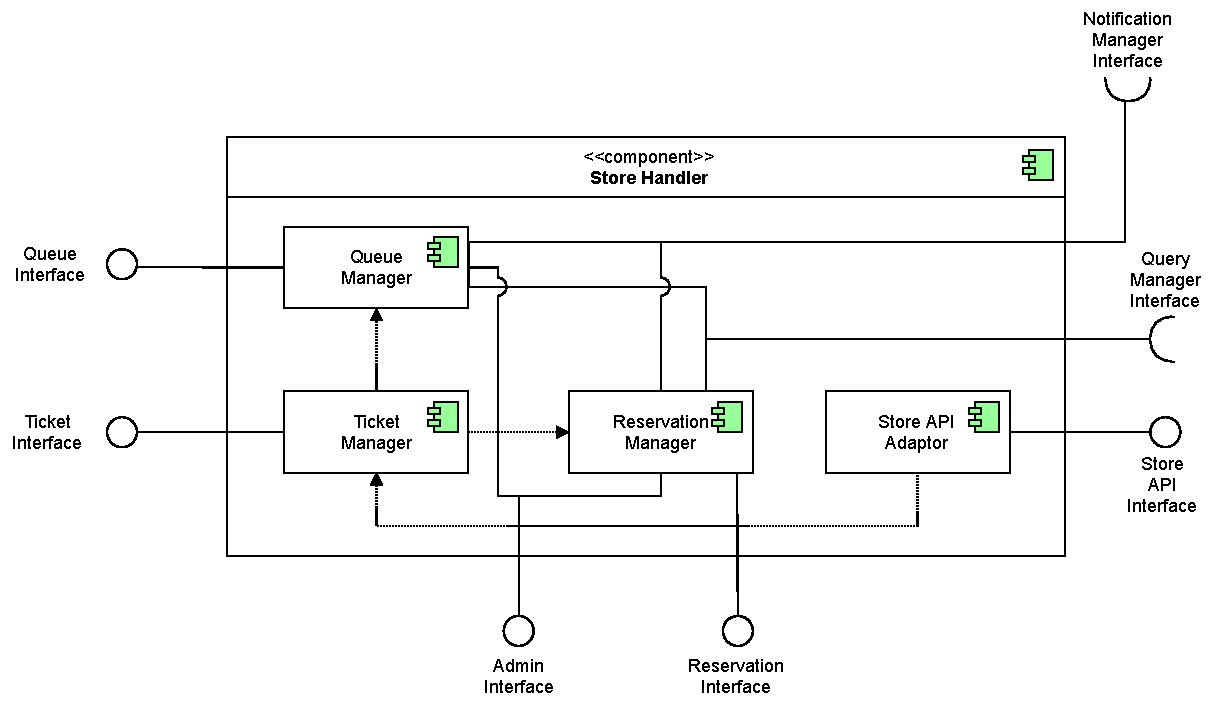
\includegraphics[width=0.8\linewidth]{images/draw.io/store_handler.pdf}
    \caption{Store Handler Internal View.\\The arrow represent a "$x$ uses $y$" relationship}
    \label{fig:store_handler}
\end{figure}

\subparagraph{Reservation Manager} is a sub-compontent of Store Handler that, for each store, allows customers to make or cancel a reservation for a certain timeslot, provides a list of available timeslot and their expected crowdness factor.

\subparagraph{Queue Manager} is a sub-component of Store Handler that, for each store, allows customers to enter or leave the virtual queue of the selected store, and provides an estimate of the waiting time.

\subparagraph{Ticket Manager} is a sub-component of Store Handler that, for each store, can receive the identifier (\emph{id}) of a queue/reservation receipt, and verifies its validity by contacting the database through \emph{Query Manager}.

\subparagraph{Store API Adaptor} is a sub-component of Store Handler that allows the system to interface with the existing infrastructure of a store, such as doors, turnstyles or cash registers, for example. It's main purpose it's to enable the system to keep track of how many customers are allowed into a store and how many exit it.

\paragraph{Notification Manager} is responsible for contacting an external notification API in order to send push notifications to client devices. It also receives User notification preference updates from the \textbf{Account Manager}. It receives state update from the \textbf{Store Handler} and dispatches notifications only to affected users.

\paragraph{Account Admin Services} is a collection (Fig. \ref{fig:admin_services}) of lower-level modules forming the features offered in the admin panel. It provides a statistical section, and a store control section, where store managers can add, edit and remove stores, their timeslots, enable or disable features such as the priority queue, or change the number of allowed customers into the store.

\begin{figure}[H]
    \centering
    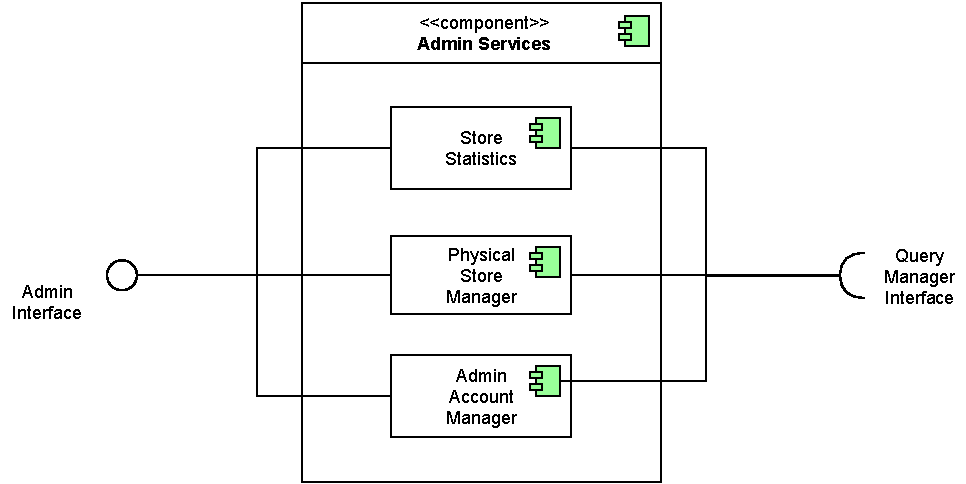
\includegraphics[width=0.8\linewidth]{images/draw.io/admin_services.pdf}
    \caption{Admin Services internal view}
    \label{fig:admin_services}
\end{figure}

\subparagraph{Store Statistics} exposes a set of functionalities targeted at extracting meaningful data from the DBMS in order to get insight on the utilization of the store and of the functionalities offered by the system, like knowing the number of people in the store at a given time or the utilization statistics of a timeslot.

\subparagraph{Physical Store Manager} is responsible for adding and removing stores. It also handles modification to store parameters such as the maximum number of people allowed, the size and the time of the timeslots, and the size of the priority queue.

\subparagraph{Admin Account Manager} is used by admins to log in to the system, and to assign managers to different stores.

\subsubsection{Data Components}
The Data layer is composed of a relational database, and its associated DBMS will have the duty of processing and executing parallel requests.

Users and Admins will be stored in different tables.
Users can set up Free Timeslots Notifications, in order to be notified when a Timeslot at a specific day in a specific time range is made available for one of the favorite stores.
Users have an association with their Tickets, which include both Queue Tickets and Reservation Tickets.
In order to preserve the history of Users and for making data analytics possible, Tickets are never deleted, but instead are associated with a status indicating if they are currently active or already used.
Each Admin manages a number of Stores, having the power of changing their capacity or all details about their associated Timeslots.
Timeslots refer to a specific weekday and have an associated time.
In order to keep consistency with Reservation Tickets, Timeslots are immutable and never modified. Their status is instead set to inactive, and another Timeslot is created whenever a change has to be made.


\begin{figure}[H]
    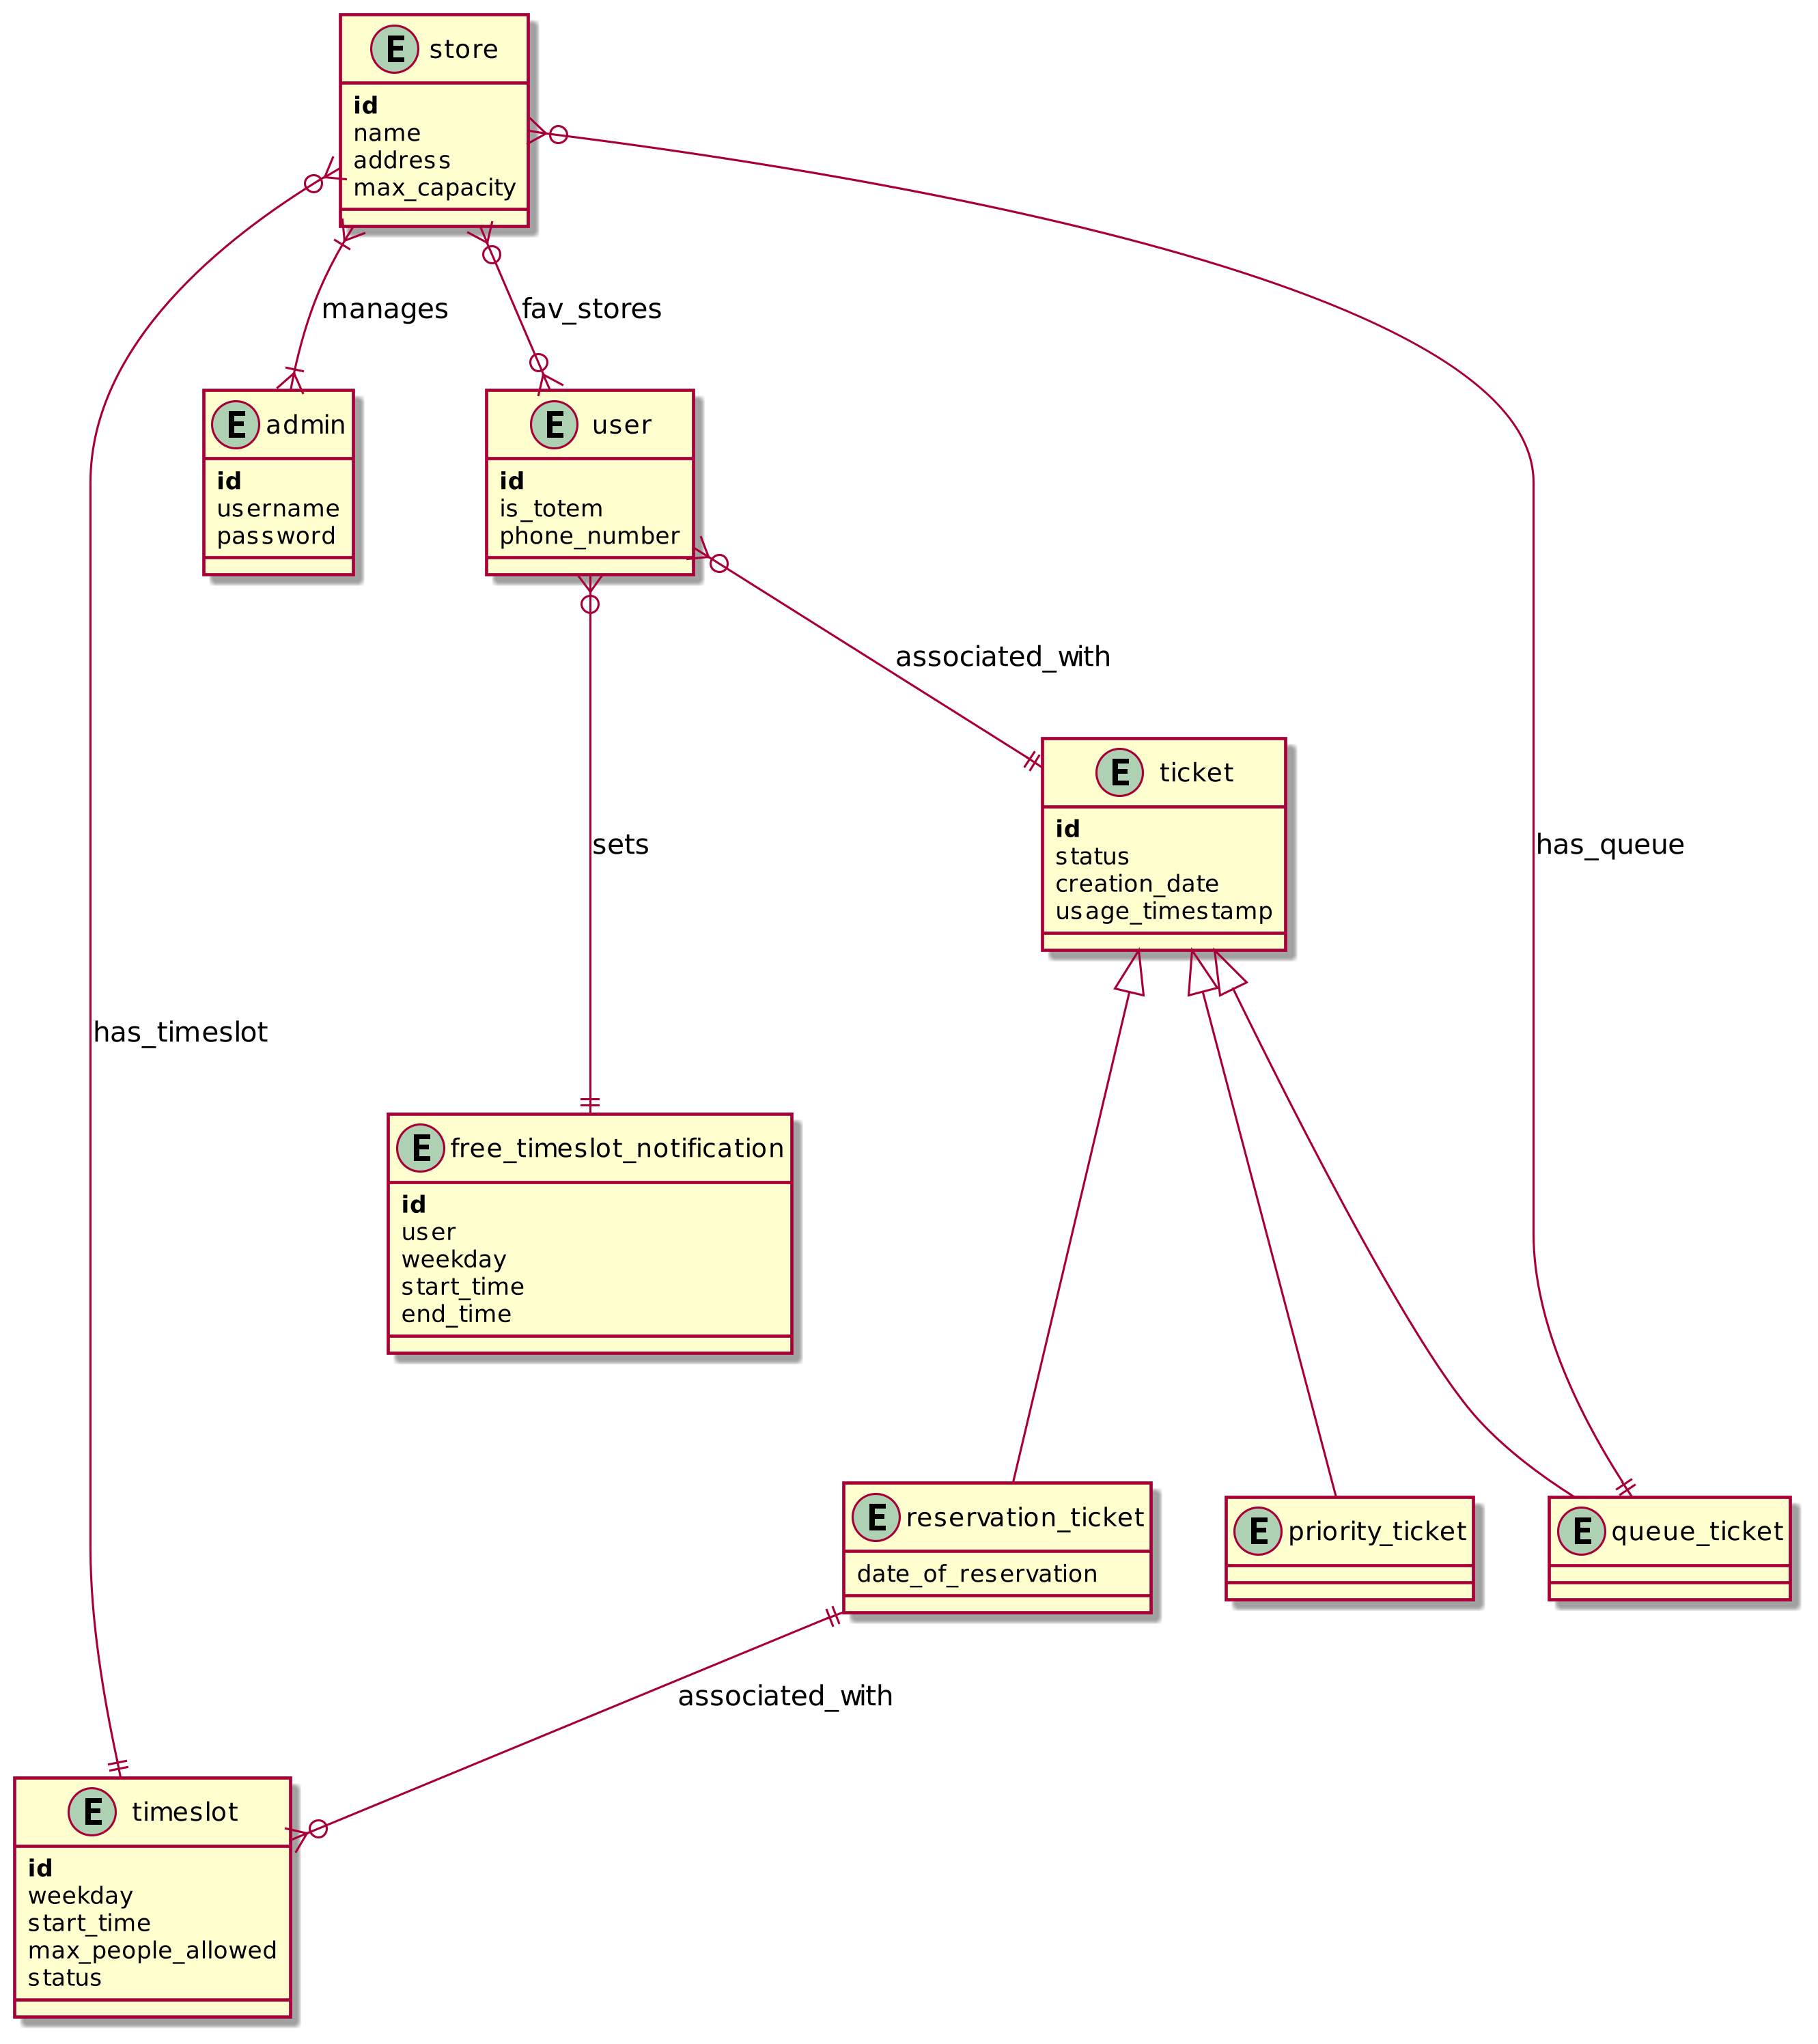
\includegraphics[width=\linewidth]{uml/db_structure.png}
    \caption{Data Base main structure}
    \label{fig:db_structure}
\end{figure}




\subsection{Deployment View}
Our system is composed of two independent components: a completely static webserver will be the access point where the client devices will fetch the one-page application, while the application server will offer the APIs to make it work.
For this reason we decided to use two different solutions.

The static webserver will make use of Cloudflare's CDN, in order to guarantee immediate response thanks to its edge location caches and reverse proxies. Cloudflare is the obvious choice as they are the major CDN providers in the world

The application server, composed of a business logic and a data tier, will be hosted on a cloud provider, offering many advantages compared to traditional in-house hosting, including:
\begin{itemize}
    \item \textbf{Scalability} thanks to the possibility of allocating new virtual machines, greater per formance cores, or more memory when needed, and to the load balancing services
    \item \textbf{Security} thanks to services like live monitoring and firewalls
    \item \textbf{Cost-Efficiency} as the great flexibility offered by the service allows for paying only the resources that are really needed.
\end{itemize}
This makes it the ideal service for hosting big and high traffic applications. The chosen cloud provider will have to offer all of the above features.

\begin{figure}[H]
    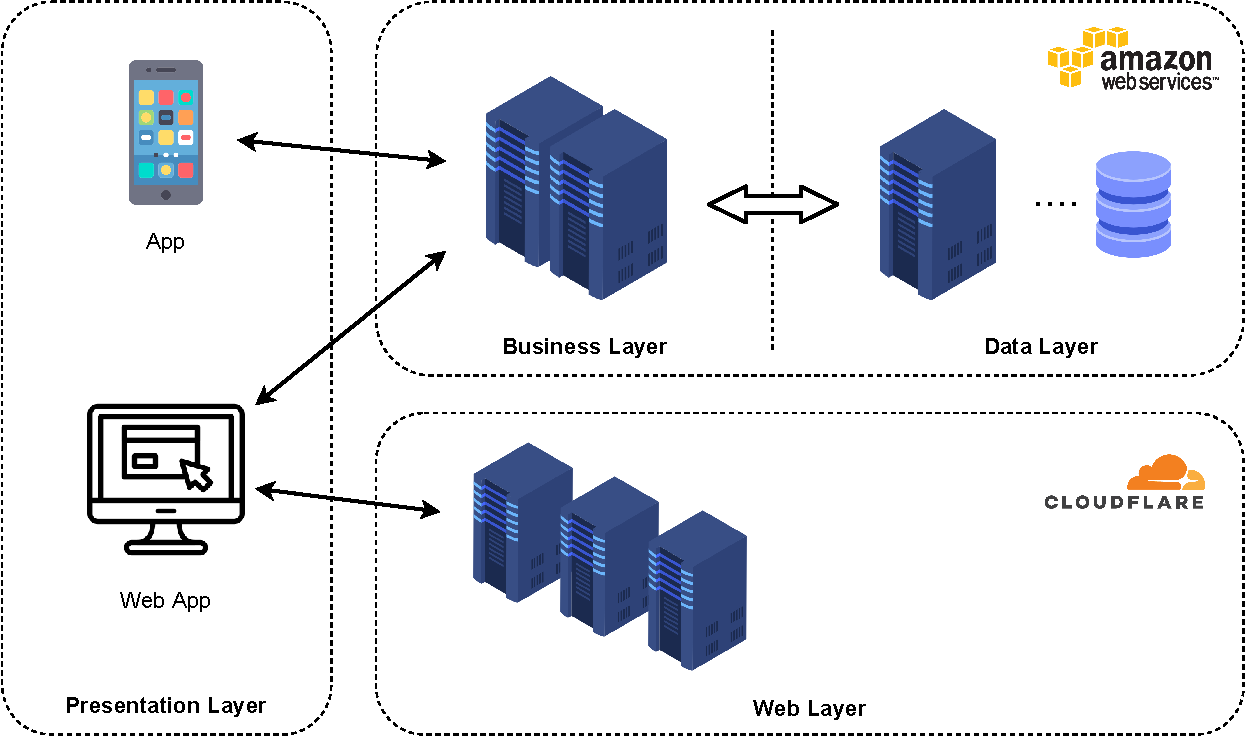
\includegraphics[width=\linewidth]{images/draw.io/deployment.pdf}
    \caption{Deployment View}
    \label{fig:deployment_view}
\end{figure}

The deployment diagram offers a clearer view over the hardware and software resources of the application:
\begin{itemize}
    \item \textbf{Mobile Device} is any device capable of hosting the mobile application, which has been previously downloaded from an official application store.
    \item \textbf{PC} is any device having a modern browser capable of running the javascript based web app.
    \item \textbf{Cloudflare CDN} will transparently host the one page application, making it available for download without impacting the performance of the main application server. No logic is implemented on this side as the application is completely static, and executes its code on the client machine.
    \item \textbf{Cloud Services} will host the entire business and data logic of the system. It contains:
    \begin{itemize}
        \item \textbf{Firewall} services for filtering incoming connections to the business and data layers
        \item \textbf{Load Balancer} service for redirecting incoming traffic to the least busy application instance
        \item \textbf{Application Instances} which will run the business logic in parallel and autonomously, and can be instantiated or deleted when needed
        \item \textbf{Data Instance} which is a data optimized virtual machine containing the DBMS and the database
    \end{itemize}
\end{itemize}

\begin{figure}[H]
    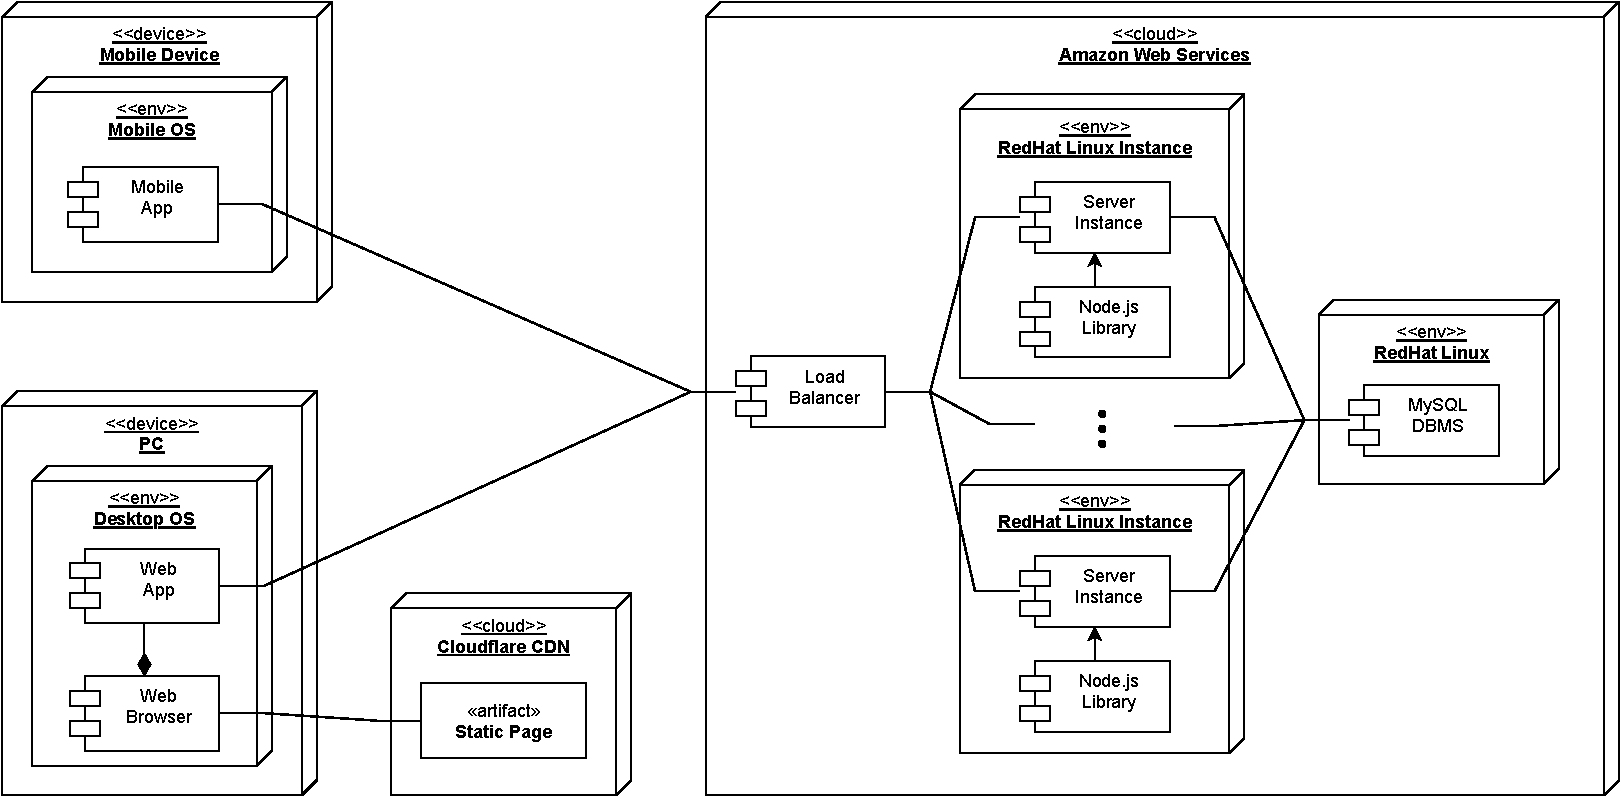
\includegraphics[width=\linewidth]{images/draw.io/deployment_structure.pdf}
    \caption{Deployment Diagram}
    \label{fig:deployment_structure}
\end{figure}

\newpage

\subsection{Runtime View}
This section describes in detail the most important runtime views of the system. Runtime views show the interaction between users and application components, showing in particular the actors involved and the specific methods called.

\begin{figure}[H]
    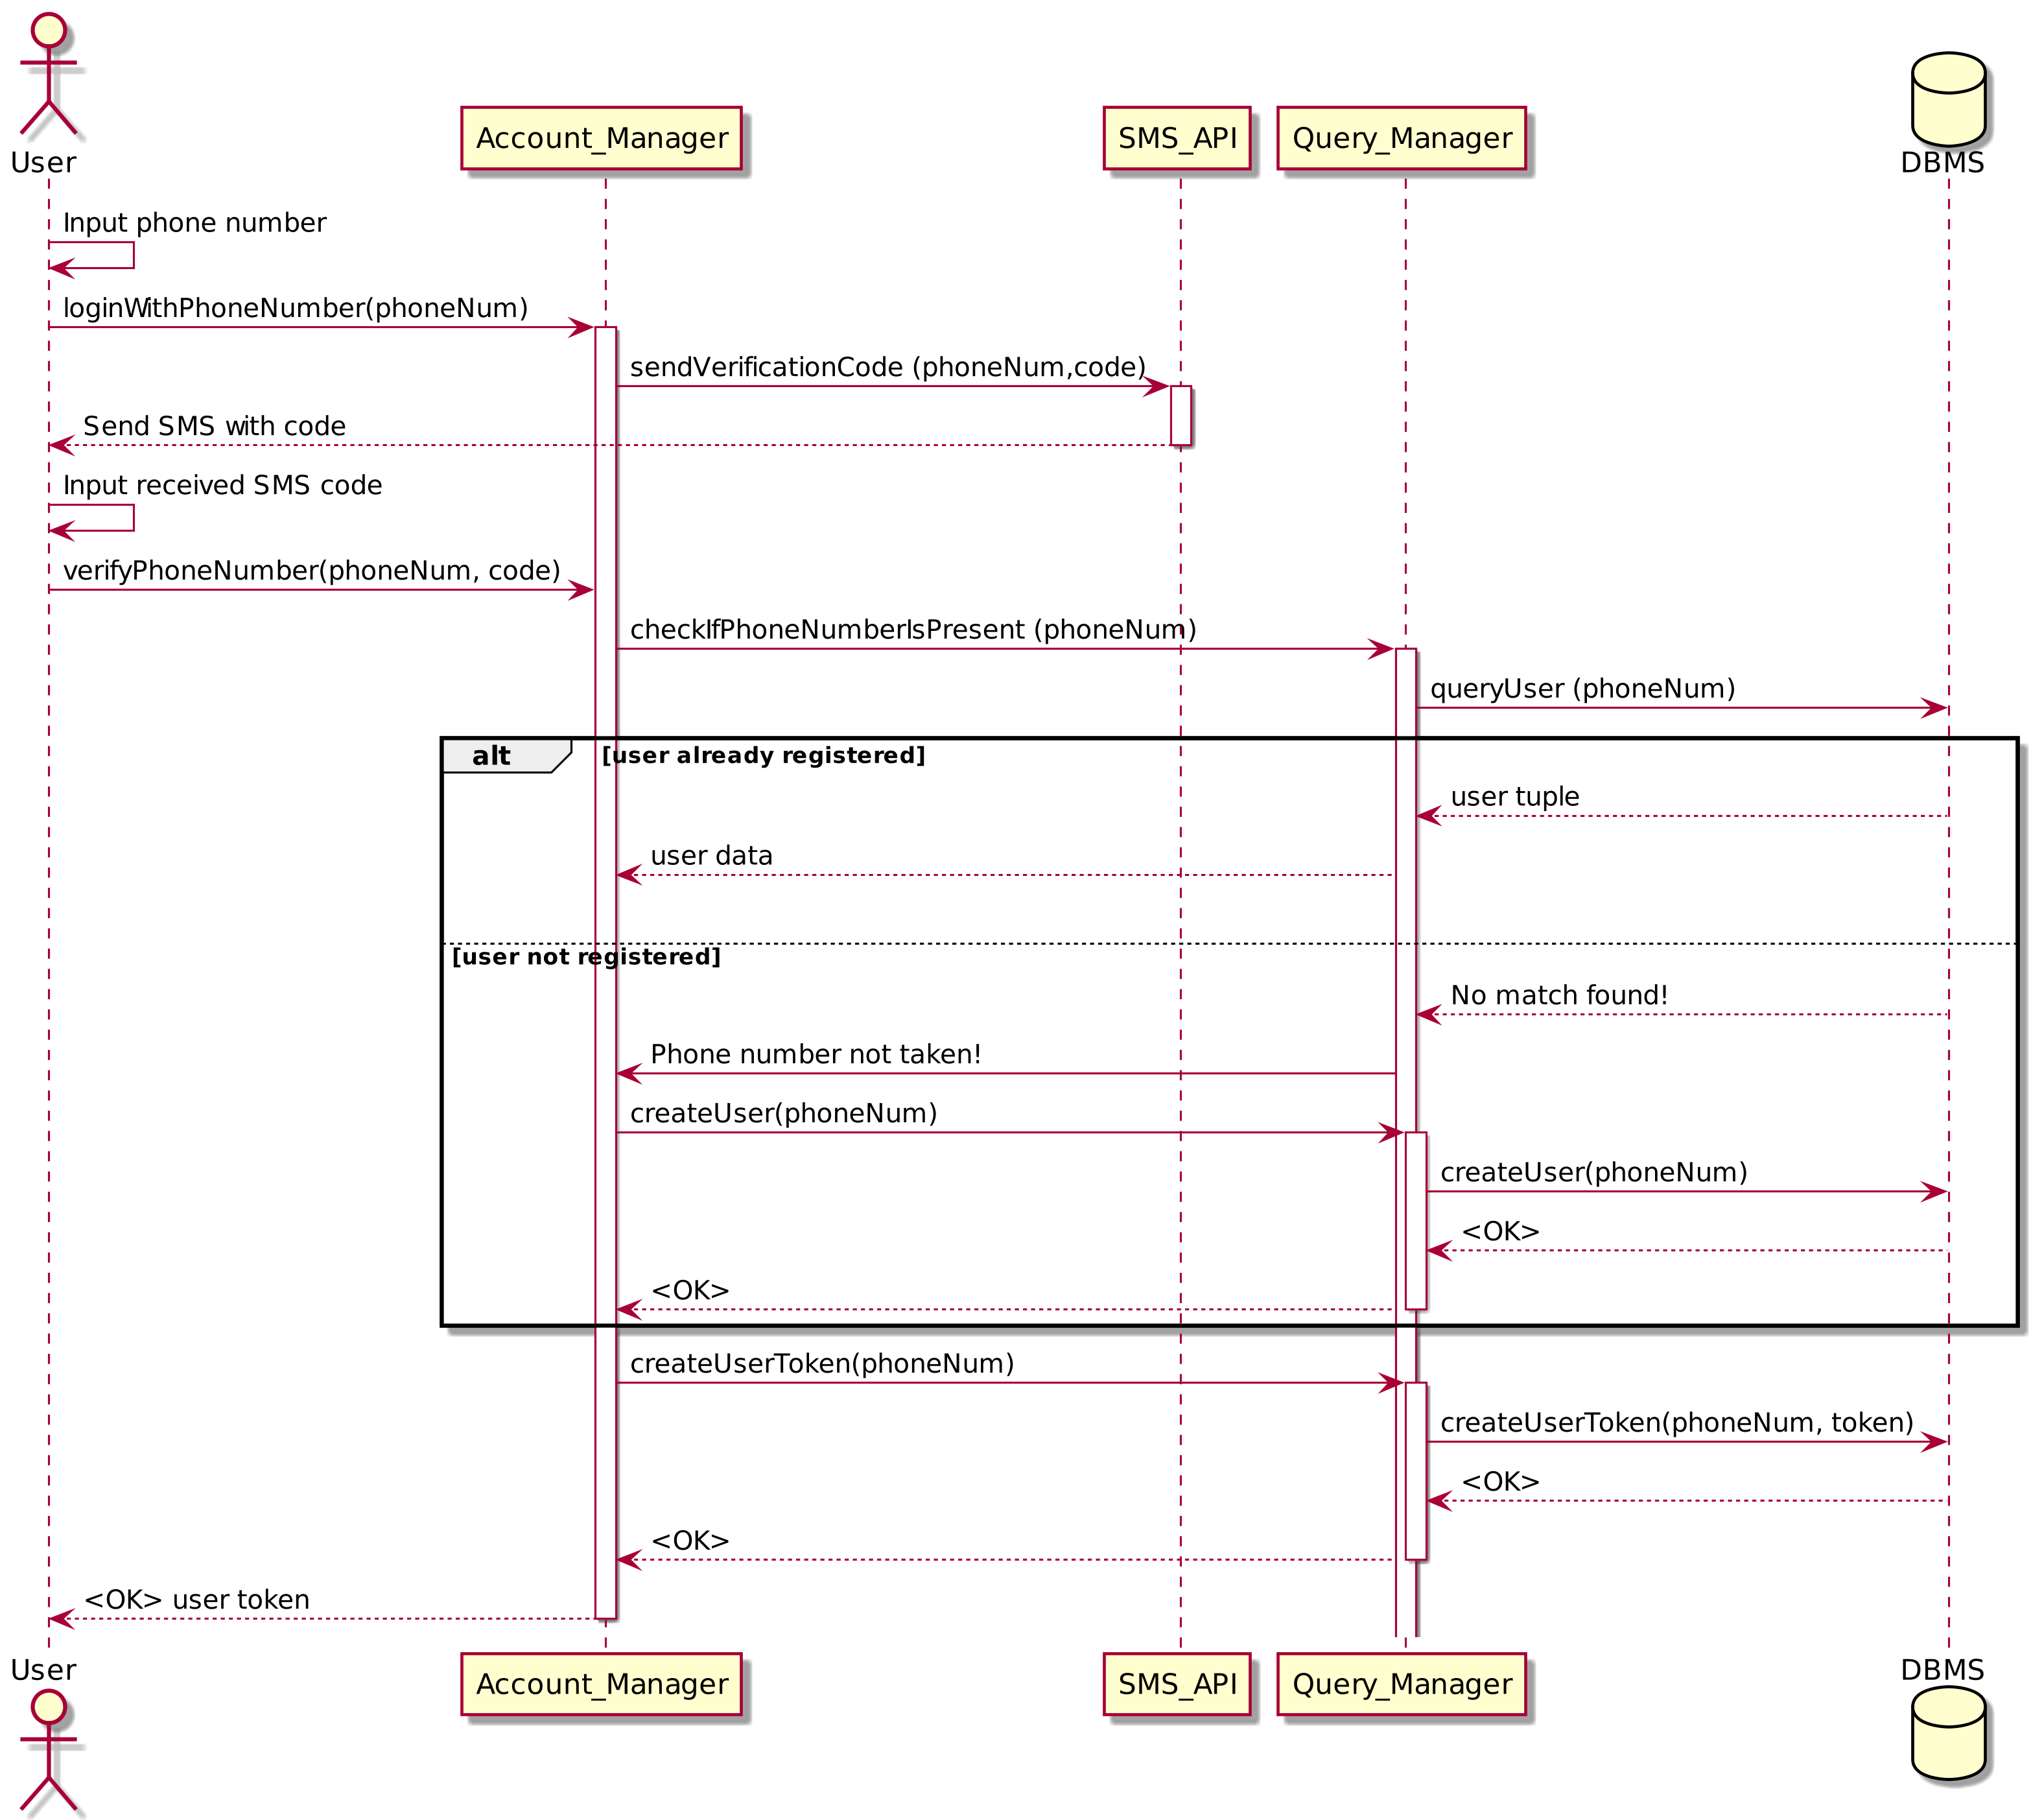
\includegraphics[width=\linewidth]{uml/seq_user_login.png}
    \caption{User Login}
    \label{fig:seq_user_login}
\end{figure}

\begin{figure}[H]
    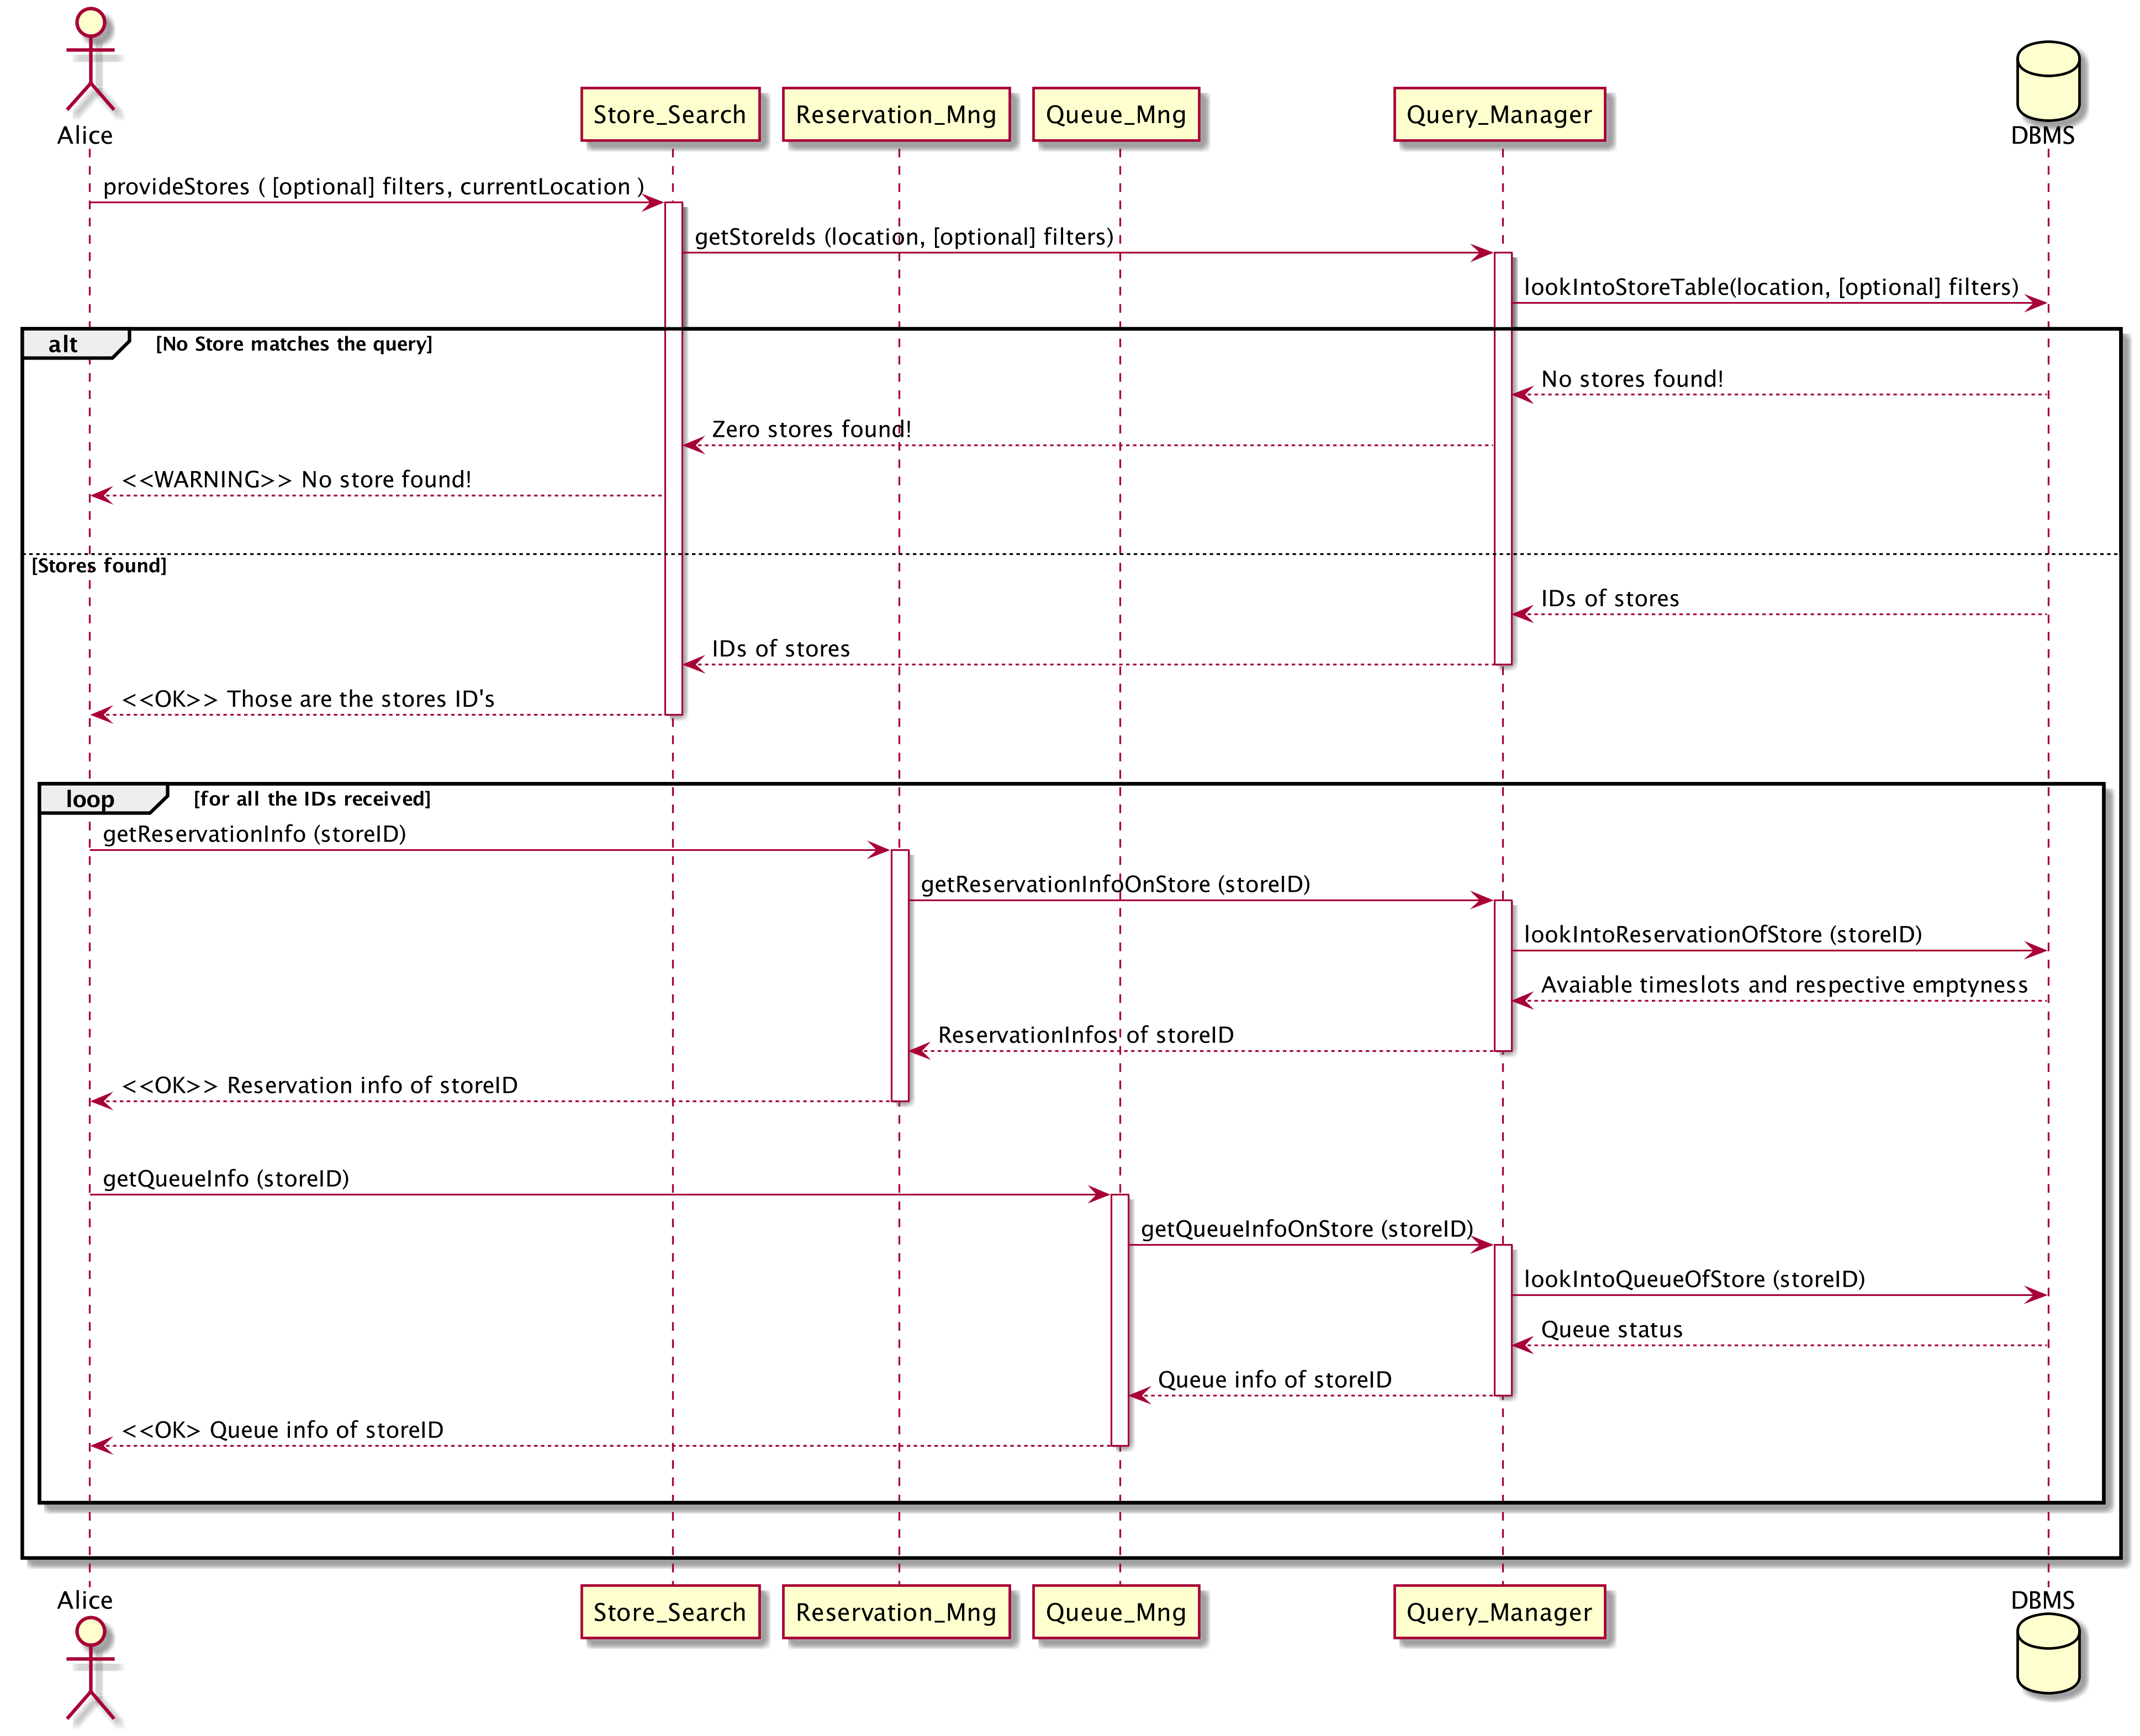
\includegraphics[width=\linewidth]{uml/seq_search_store.png}
    \caption{Store search}
    \label{fig:seq_store_search}
\end{figure}

\begin{figure}[H]
    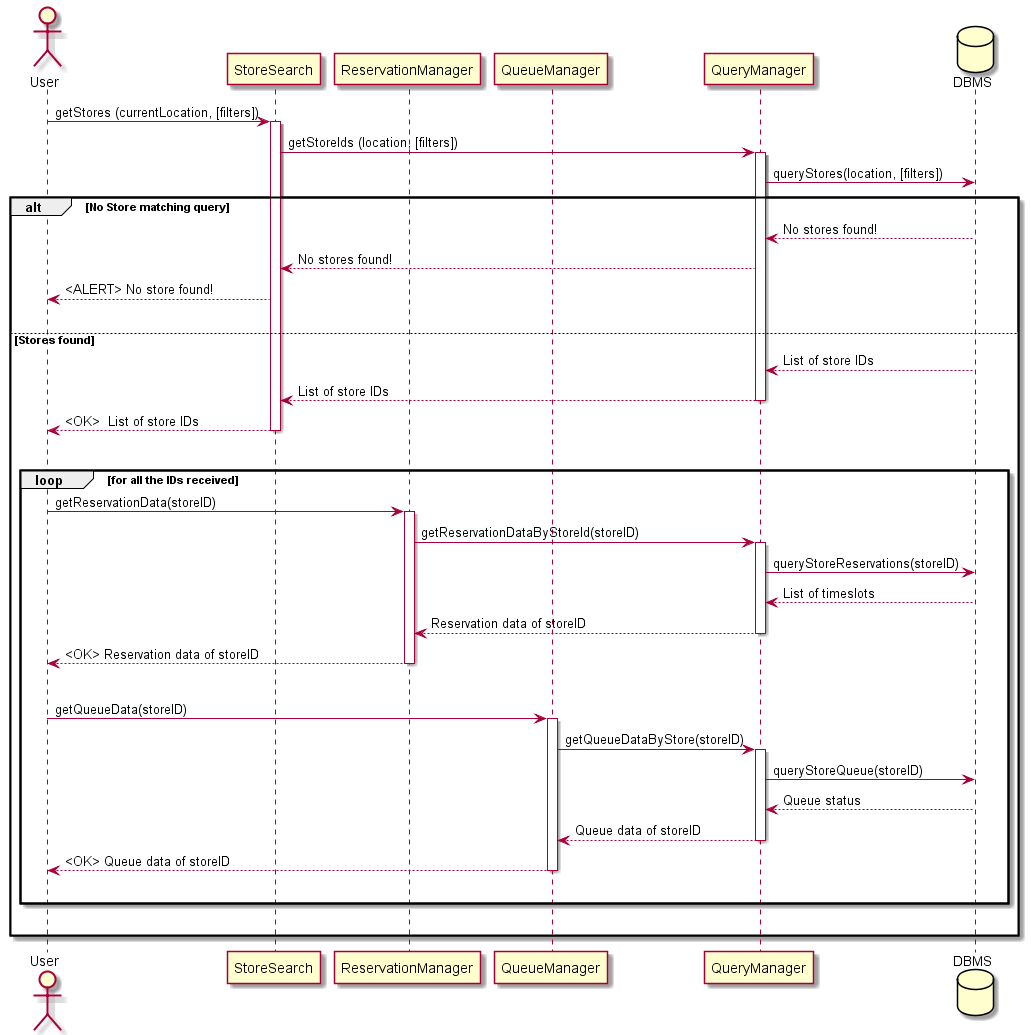
\includegraphics[width=\linewidth]{uml/seq_join_queue.png}
    \caption{User joins queue}
    \label{fig:seq_join_queue}
\end{figure}


\begin{figure}[H]
    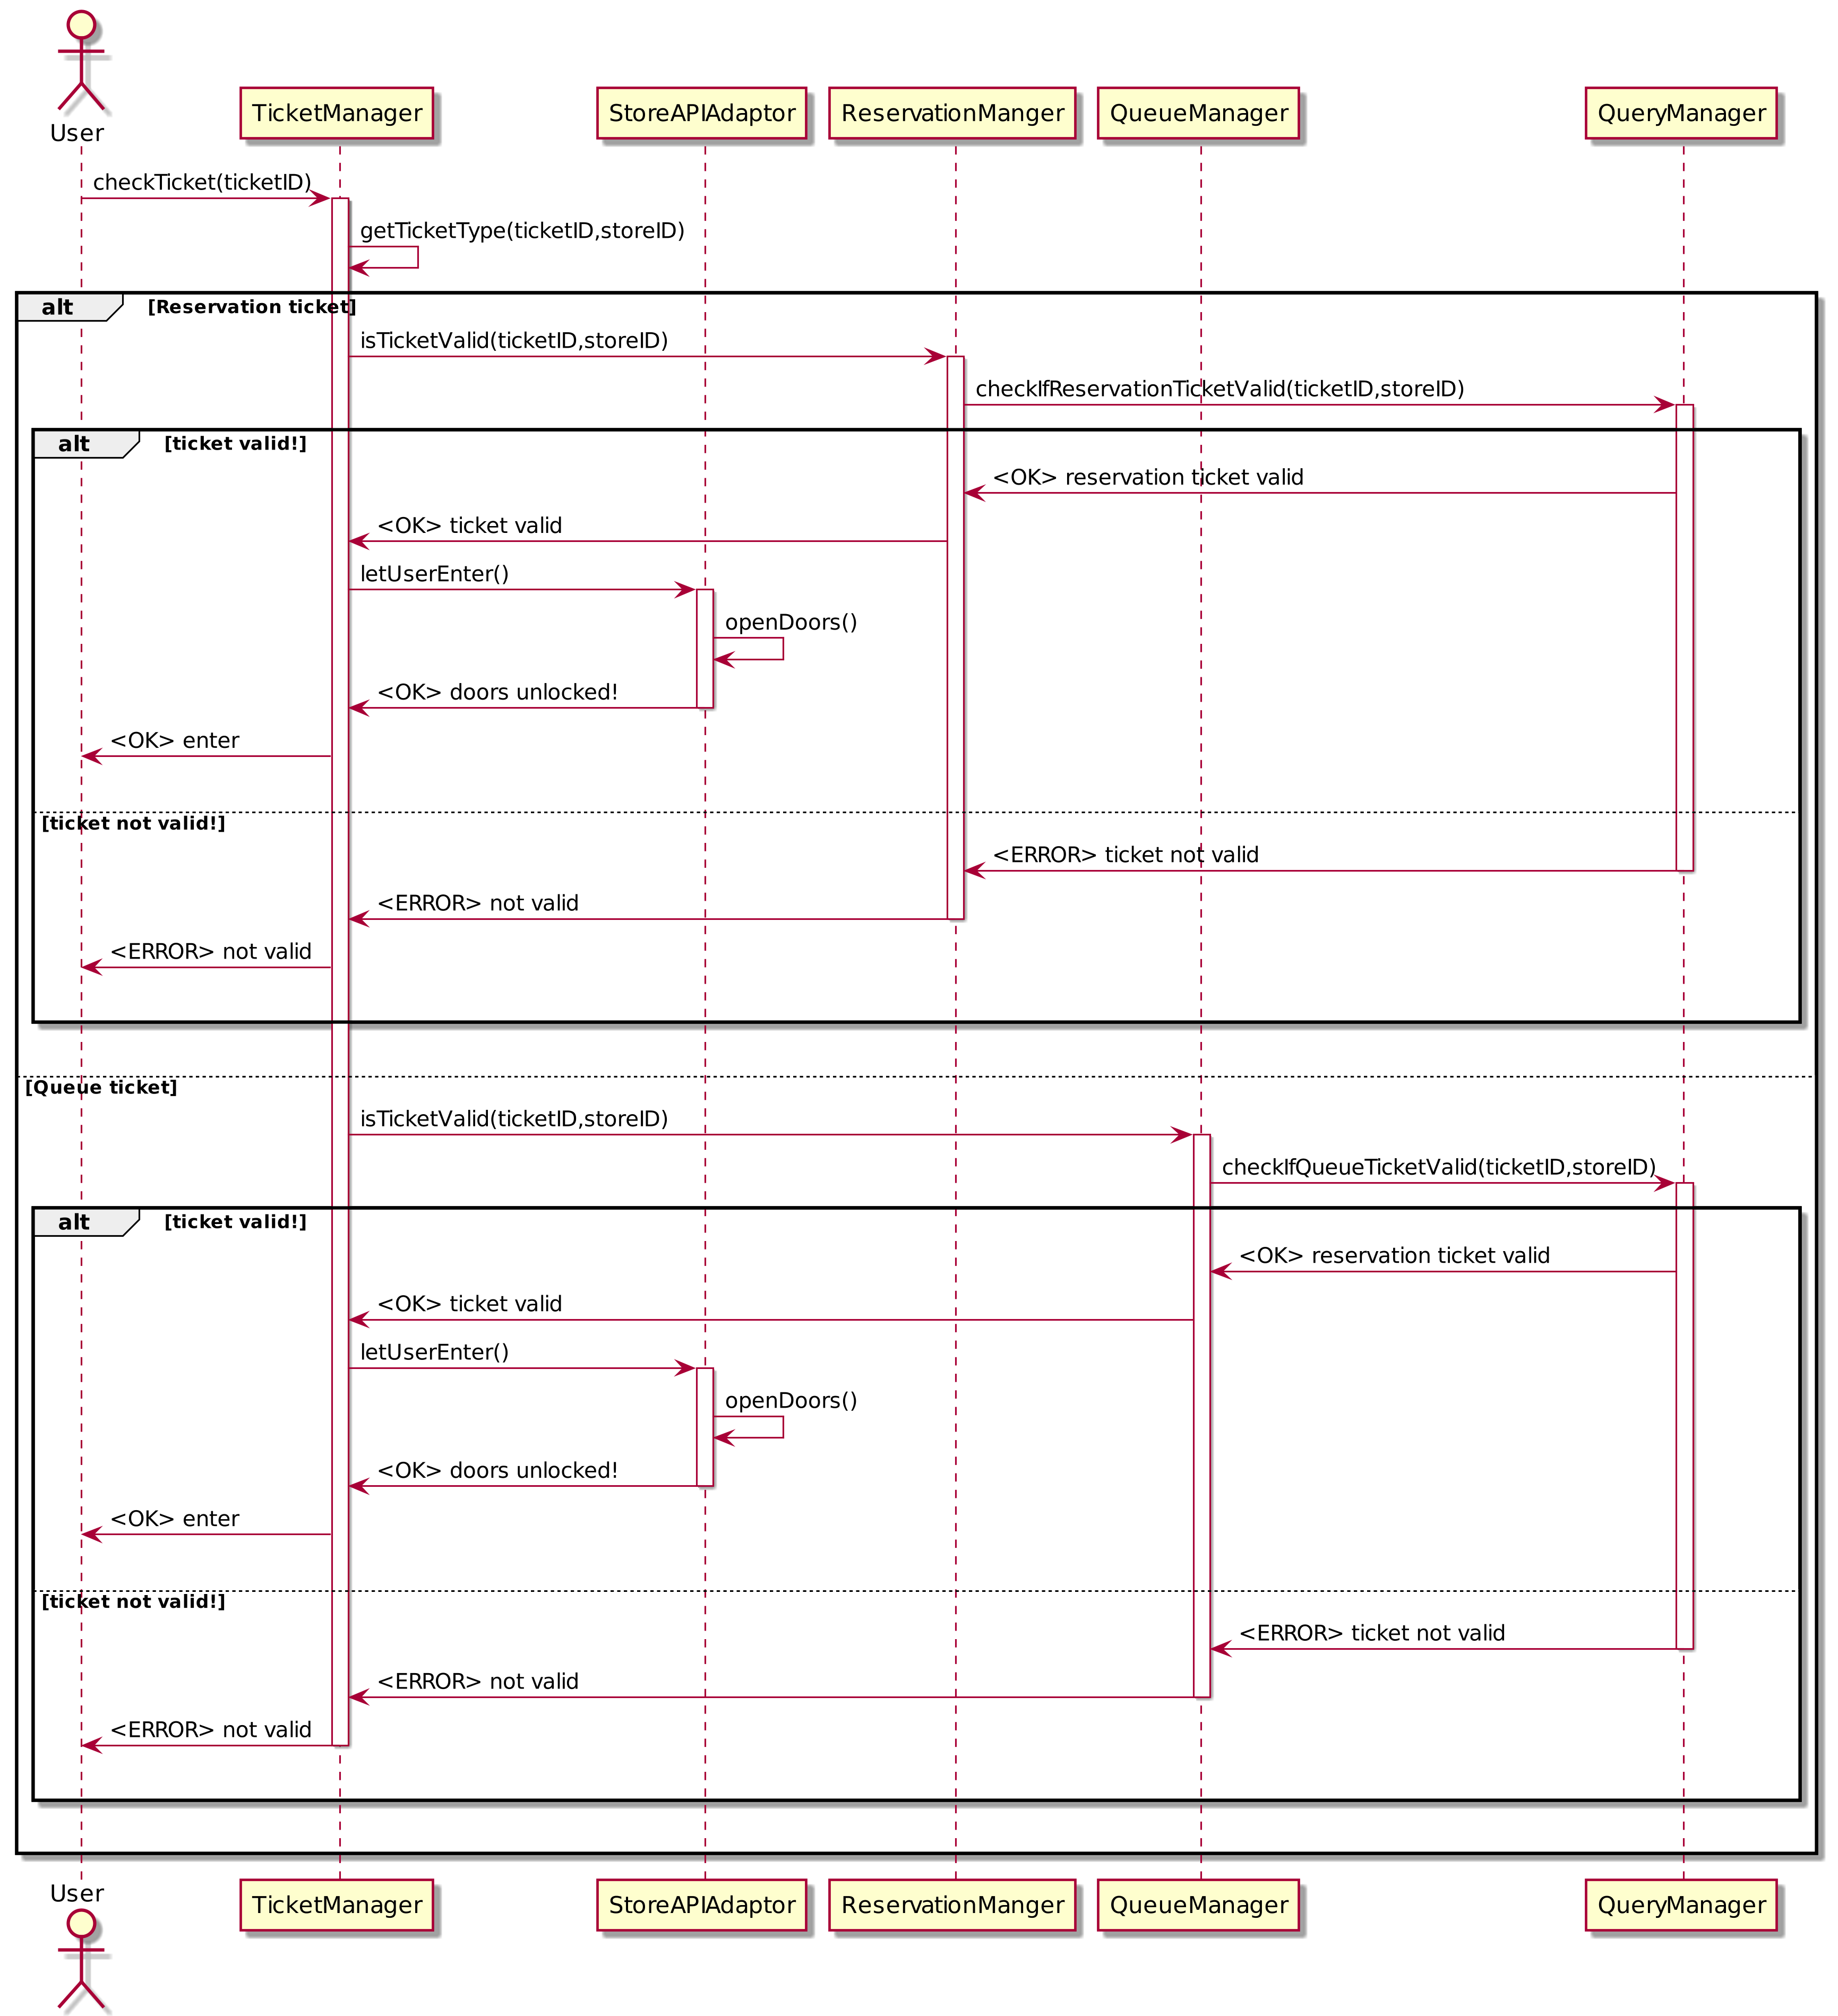
\includegraphics[width=\linewidth]{uml/seq_user_enters_store.png}
    \caption{User access the store - Data Base is omitted for clarity}
    \label{fig:seq_user_access_store}
\end{figure}

\begin{figure}[H]
    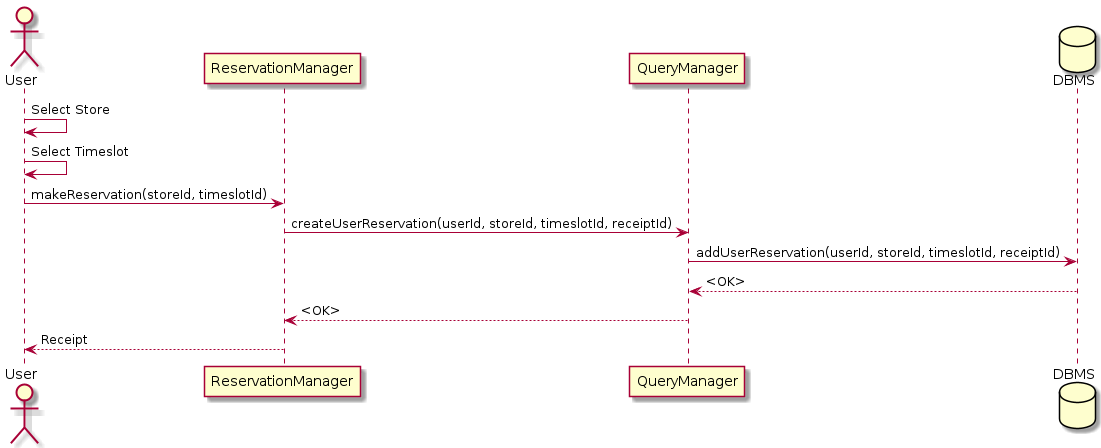
\includegraphics[width=\linewidth]{uml/seq_make_reservation.png}
    \caption{User makes a reservation}
    \label{fig:seq_make_reservation}
\end{figure}
 
\begin{figure}[H]
    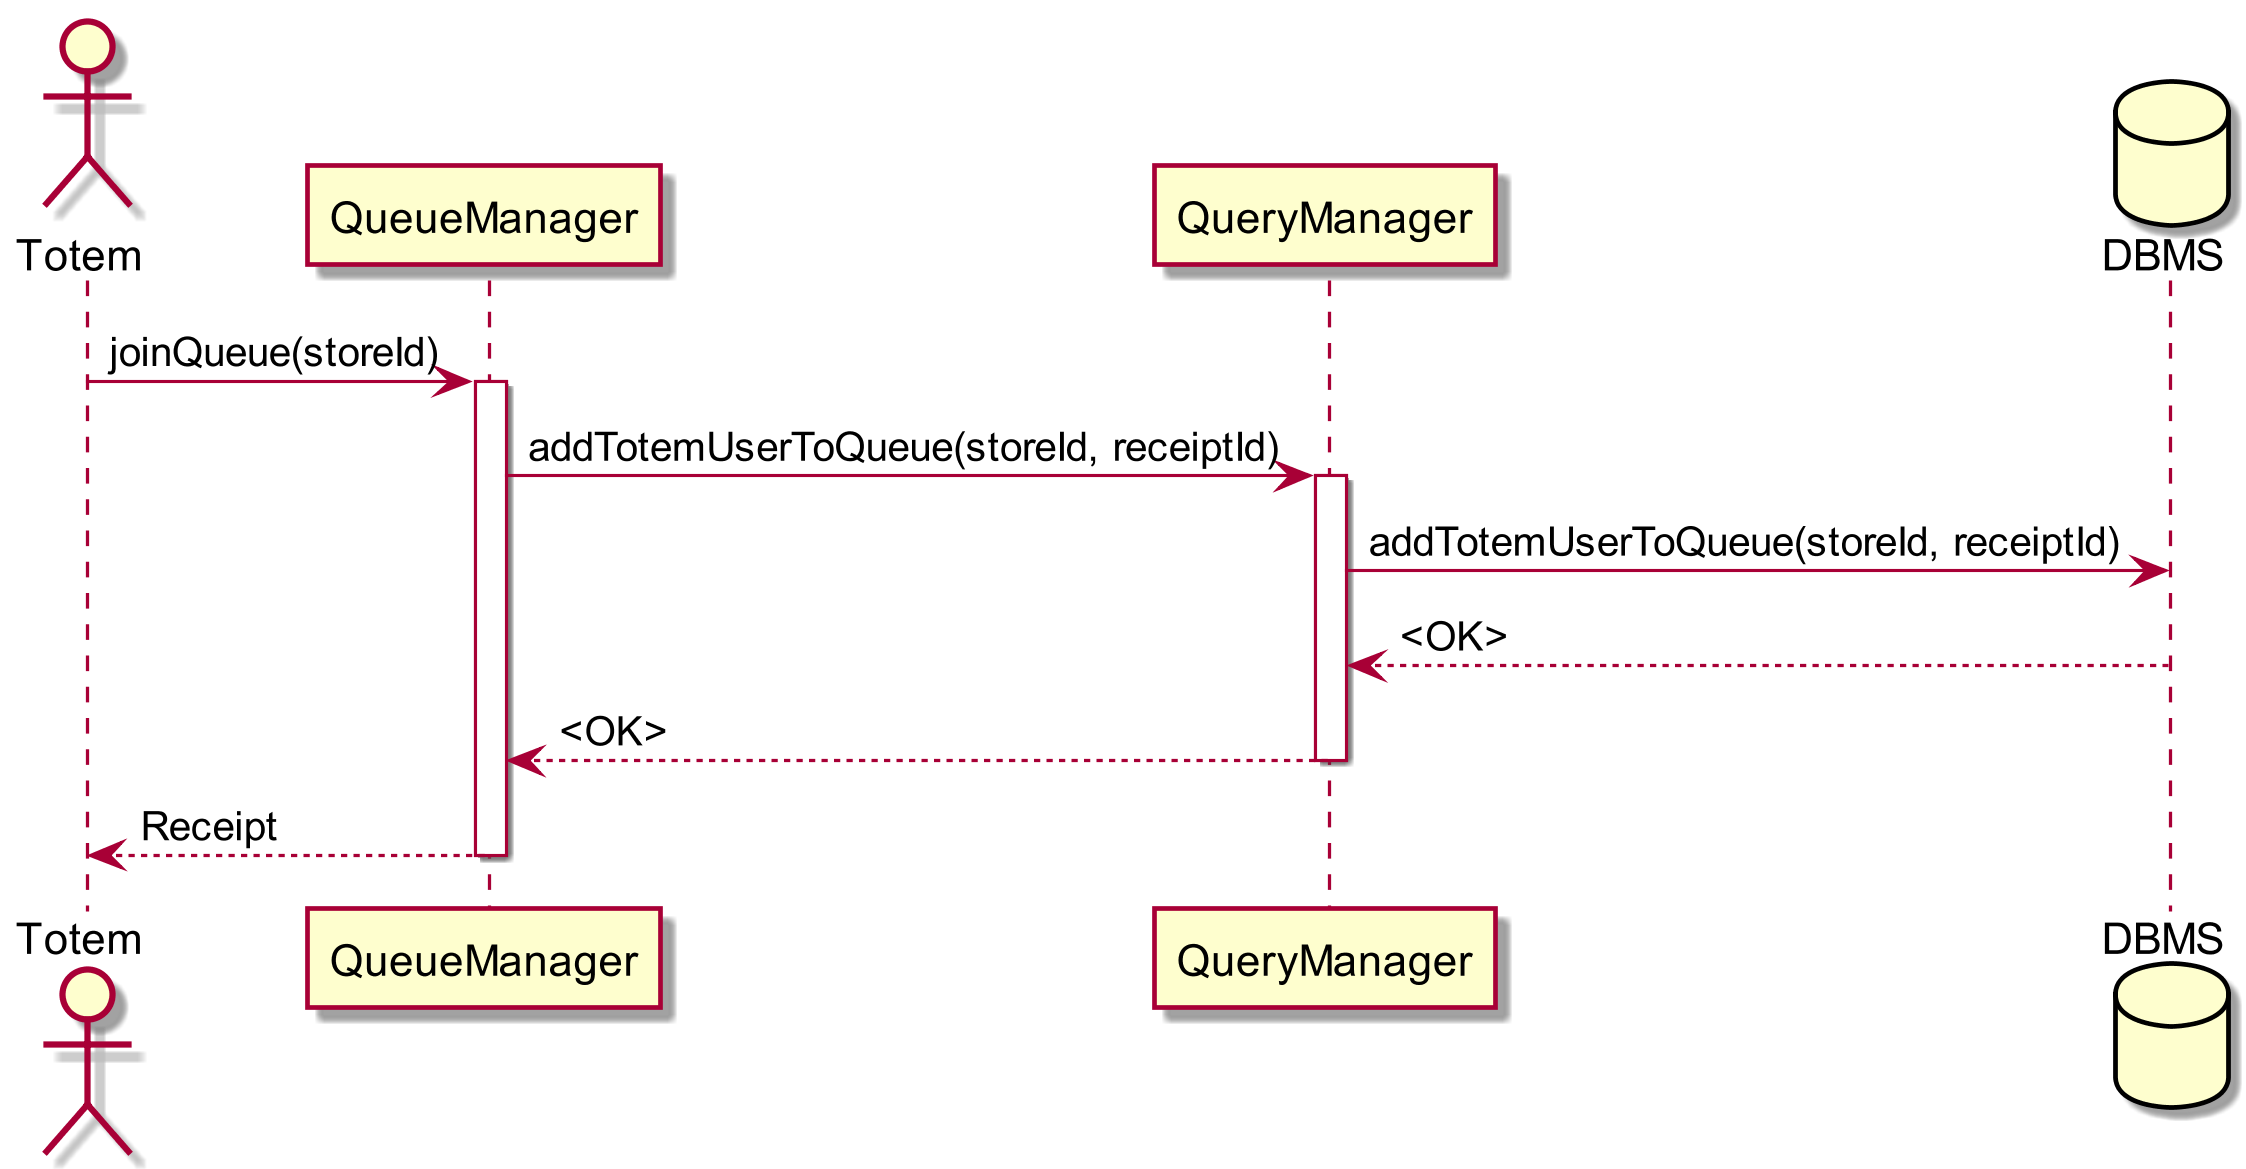
\includegraphics[width=\linewidth]{uml/seq_join_queue_totem.png}
    \caption{User joins the queue from the totem}
    \label{fig:seq_join_queue_totem}
\end{figure}

\begin{figure}[H]
    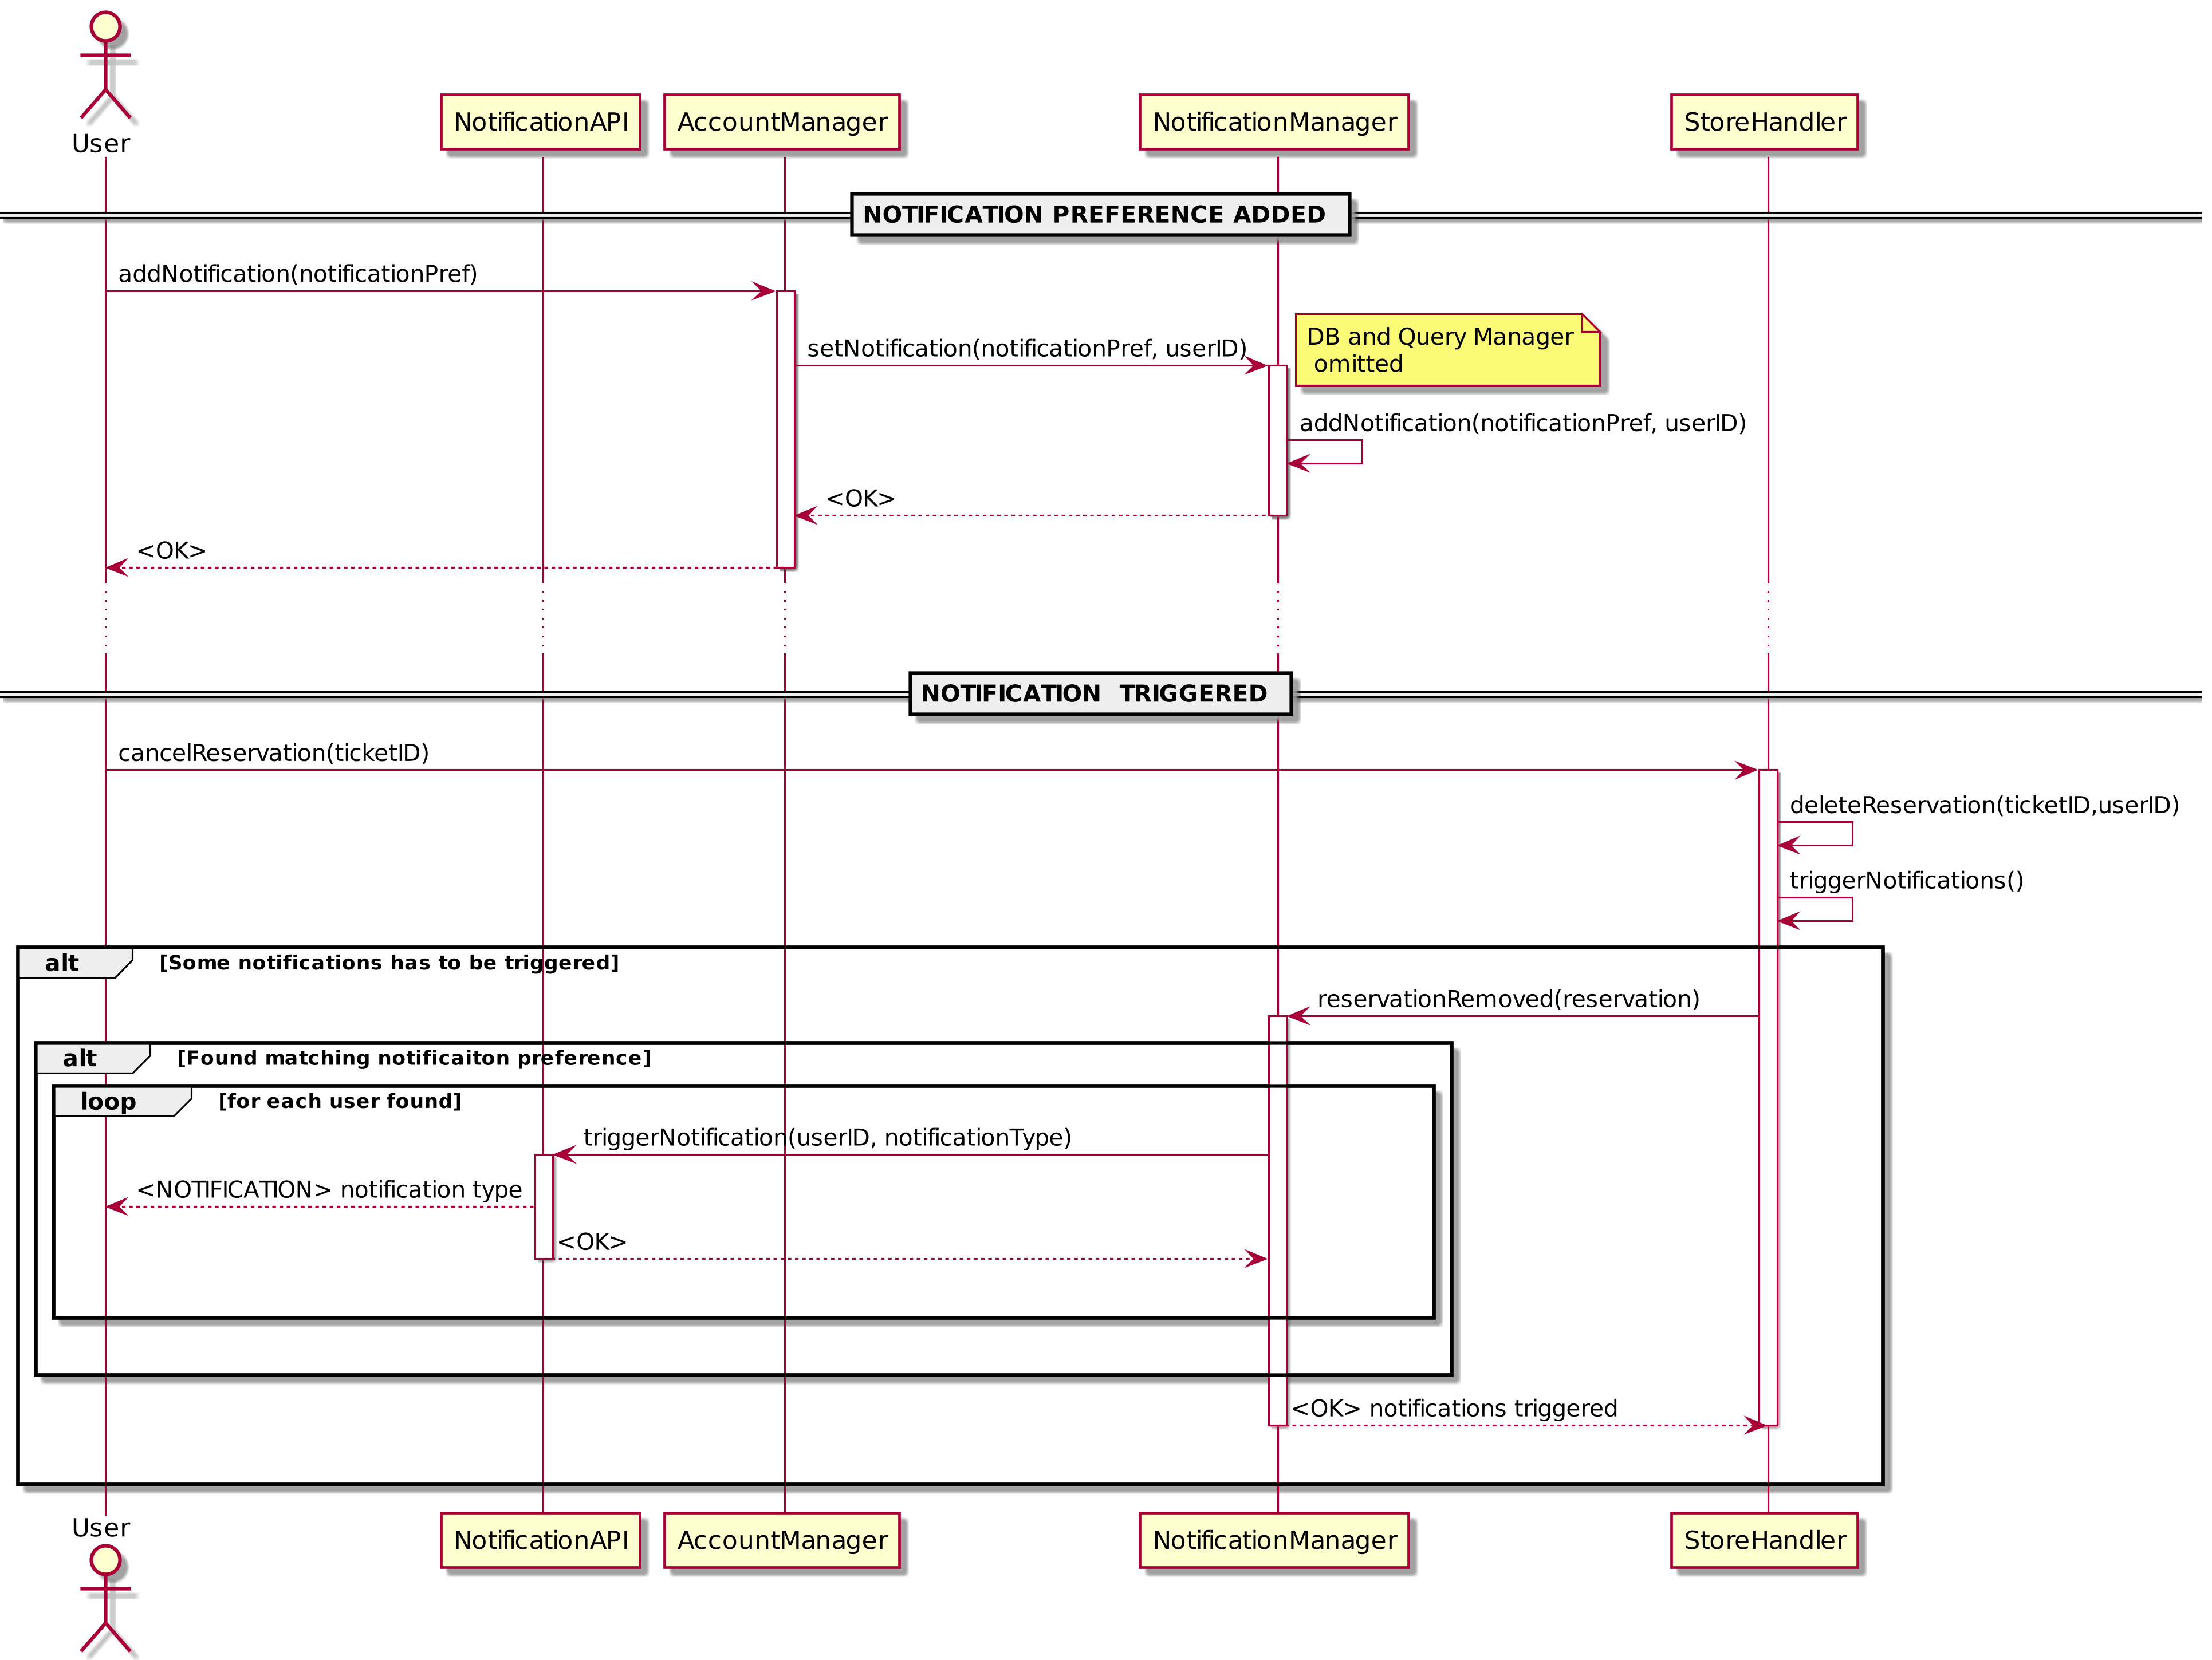
\includegraphics[width=\linewidth]{uml/seq_user_gets_notified.png}
    \caption{User sets a notification - User is notified}
    \label{fig:seq_user_gets_notified}
\end{figure}

\begin{figure}[H]
    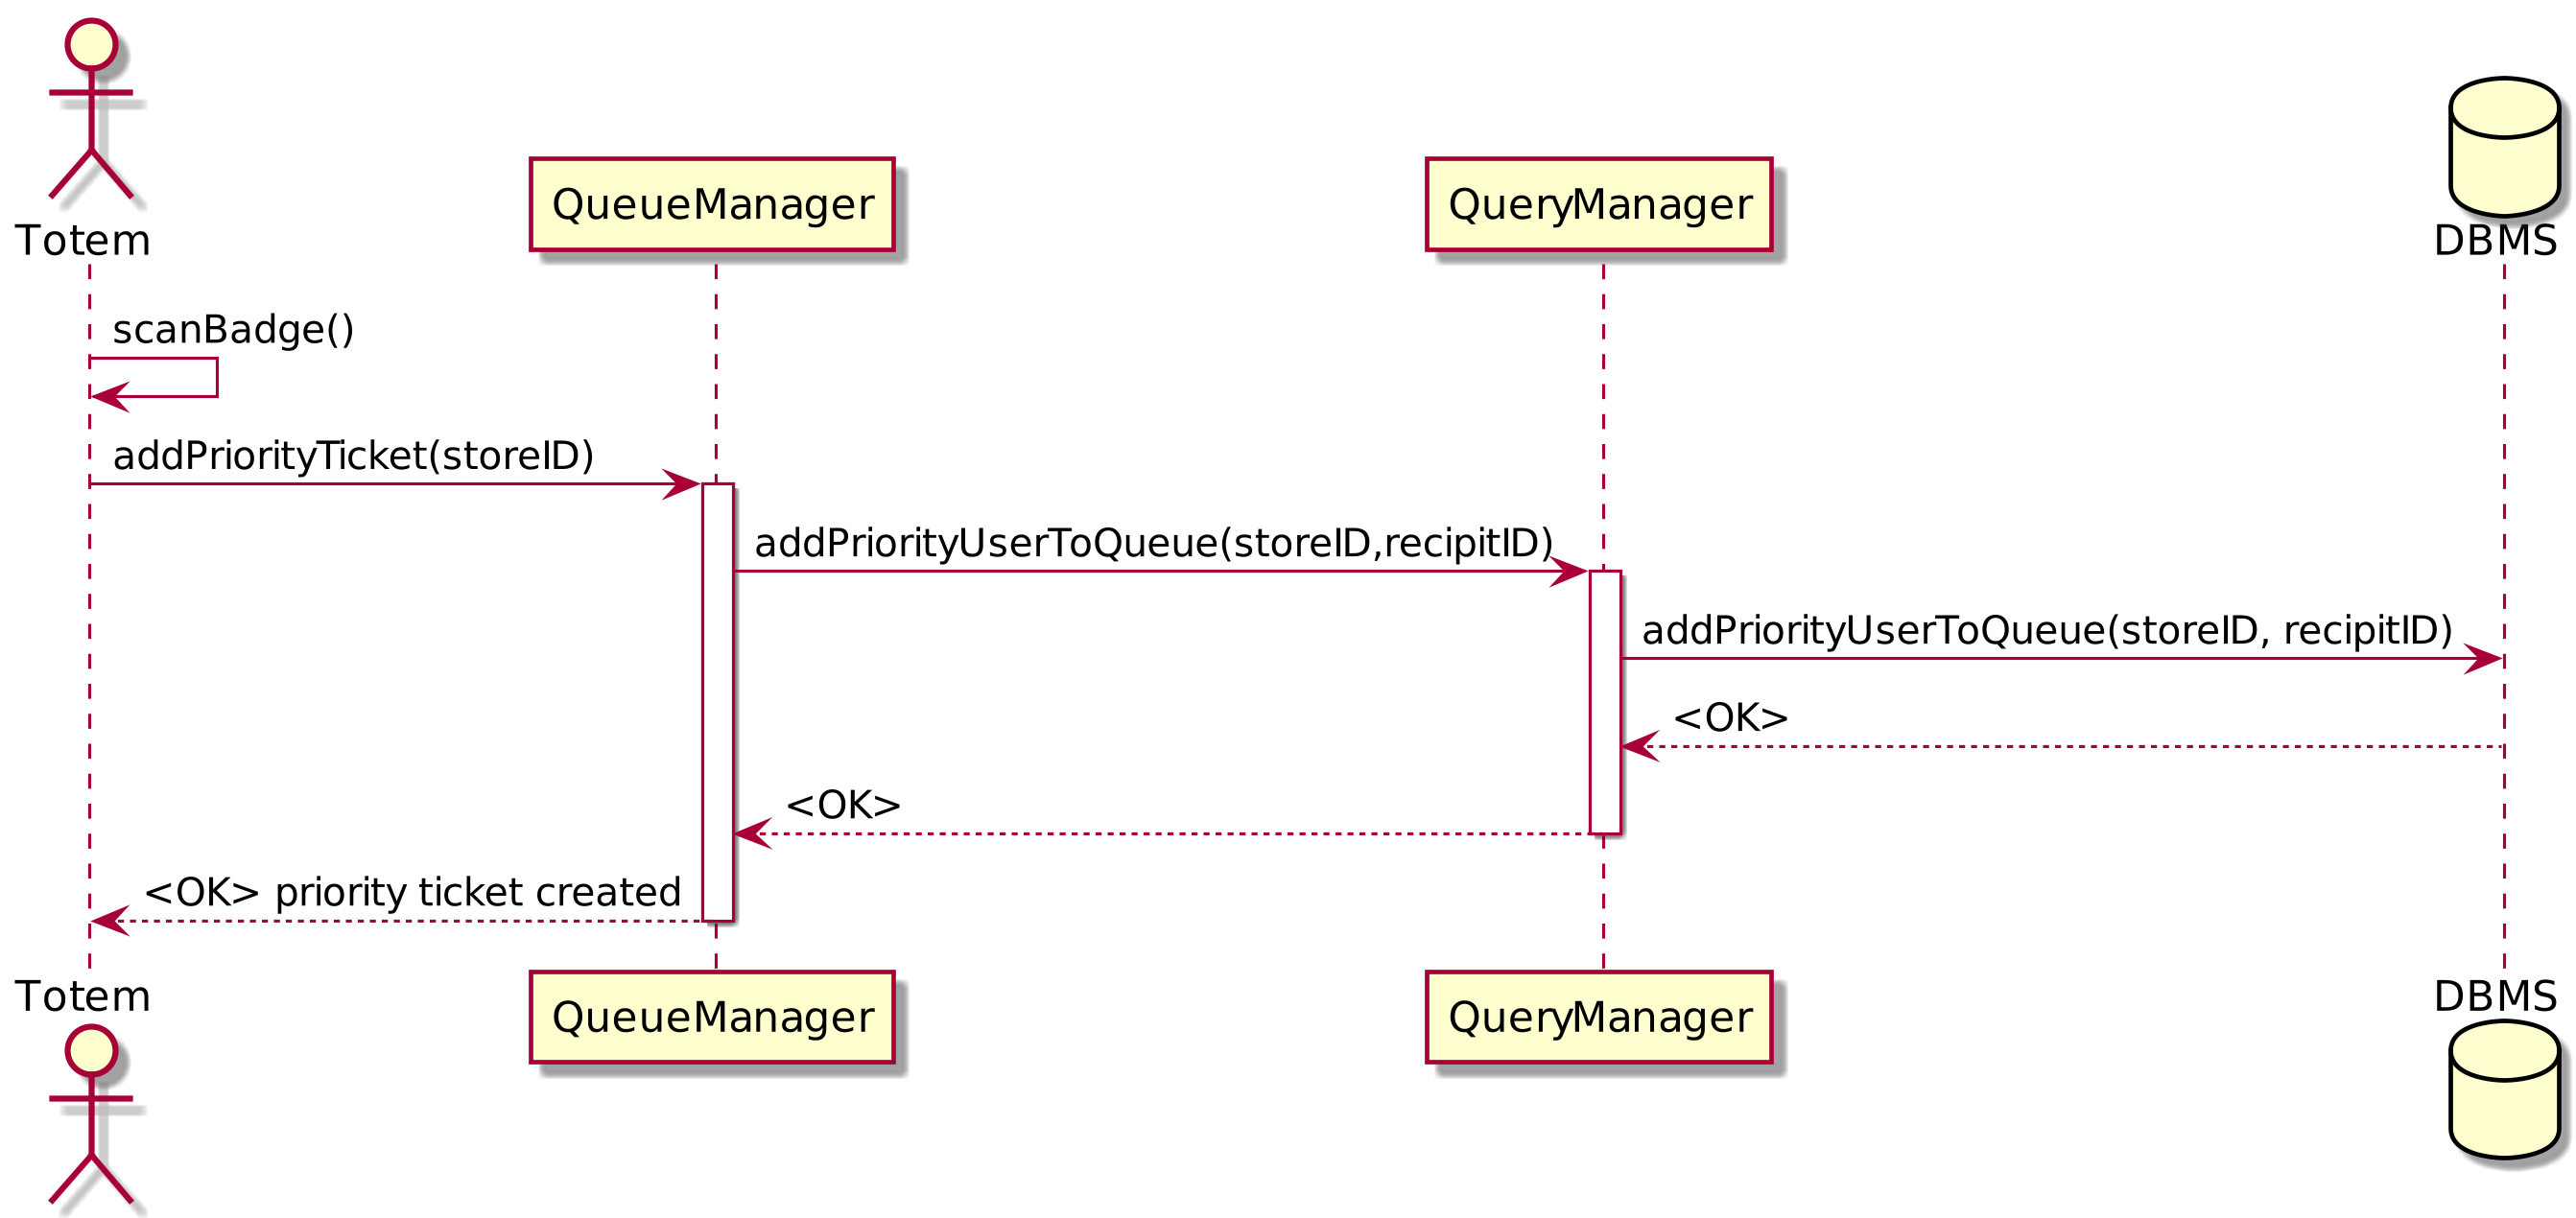
\includegraphics[width=\linewidth]{uml/seq_priority_ticket_creation.png}
    \caption{Employee creates priority ticket}
    \label{fig:seq_priority_ticket}
\end{figure}

\newpage

\subsection{Component Interfaces}
In this section we will describe the most relevant interfaces exposed by the components, including all the ones seen in Fig. \ref{fig:component}.

\begin{itemize}
    \item \textbf{QueryManager}
    \begin{itemize}
        \item \textbf{checkIfPhoneNumberIsPresent(phoneNum)}
        This method takes as an input the phone number of the user (phoneNum) and contacts the DBMS to check if the phone number is already present in the system. A reply is then sent to the caller.

        \item \textbf{createUser(phoneNum)}
        This method takes as an input the phone number (phoneNum) of the user to be created and adds it to the DBMS. A reply is then sent to the caller.

        \item \textbf{createUserToken(phoneNum)}
        This method takes as an input the phone number (phoneNum) of the user that is trying to login into the system and it generates the token associated with its session. Saving those information in the DBMS. A reply is then sent to the caller.

        \item \textbf{validateToken(token)}
        This method takes as an input the token passed by the user in every request and checks if it is valid and corresponds to an active session. A reply is then sent to the caller.

        \item \textbf{getStoreIds(location, [filters])}
        This method takes as input the location provided by the User and an optional list of filters. 
        The QueryManager will retrive the stores respecting those constrains by the means of the DBMS. A reply is then sent to the caller. 

        \item \textbf{getReservationDataByStoreID(storeID)}
        This method takes as input the store identification number. The QueryManager will acquire from the DBMS the informations regarding the reservation overall status of the given storeID. A reply is then sent to the caller.

        \item \textbf{getQueueDataByStore(storeID)}
        This method takes as input the store identification number. The QueryManager will acquire from the DBMS the informations regarding the queue overall status of the given storeID. A reply is then sent to the caller. 

        \item \textbf{addUserToQueue(userID, storeID, receipitID)}
        This method takes as input the identification number of the user, the store, and the recepit. 
        It adds those values to the dedicated table in the DBMS. A reply is then sent to the caller.

        \item \textbf{addTotemUserToQueue(storeID, receipitID)}
        This method takes as input the receipt identification number of the ticket generated by the QueueManager and the unique store id number of the store where the ticket is generated. It adds those values to the dedicated table in the DBMS. The user identification number is not present as a parameter, since no registration is required to join the queue from a totem. An anonymous entry will be added to the DBMS table. A reply is then sent to the caller. 
        \item \textbf{createUserReservation(userID, storeID, timeslotID, receipitID)}
        This method takes as input the identificaton number of the user, the store, the selected timeslot and the recipit. It adds those values to the dedicated table in the DBMS. A reply is then sent to the caller. 
        \item \textbf{checkIfReservationTickeValid(tickedID, storeID)}
        This method takes as an input the identification number of the provided ticket and the store.
        It checks if those values are present in the Reservation table by the means of the DBMS. A reply is the sent to the caller.  
        \item \textbf{checkIfQueueTickeValid(tickedID, storeID)}
        This method takes as an input the identification number of the provided ticket and the store.
        It checks if those values are present in the Queue table by the means of the DBMS. A reply is the sent to the caller. 
        

    \end{itemize}

    \item \textbf{ReservationManager}
    \begin{itemize}
        \item \textbf{getReservationData(storeID)}
        This method takes as an input the store identification number and contacts the QueryManager to get the reservation data on the specified store id. A reply is then sent to the caller.

        \item \textbf{isTicketValid(ticketID,storeID)}
        This method takes as input the identification number of the ticket and the store. It checks by contacting the QueryManager if the provided ticket is currently valid for the selected store. 
        A reply is then sent to the caller. 

        \item \textbf{makeReservation(storeID,timeslotID)}
        This method takes as input the identification number of the store and of the timeslot. The ReservationManager will then contact the QueryManager to insert the reservation into the system. The user identification number is provided within the session of the current user. A reply is then sent to the caller. 

        \item \textbf{cancelReservation(ticketID)}
        This method takes as input the identification number of the ticket. It removes the associated reservation. 
        A reply is then sent to the caller. 
    \end{itemize}

    \item \textbf{QueueManager}
    \begin{itemize}
        \item \textbf{getQueueData(storeID)}
        This method takes as an input the store identification number and contacts the QueryManager to get the queue data on the specified store id. A reply is then sent to the caller.

        \item \textbf{isTicketValid(ticketID,storeID)}
        This method takes as input the identification number of the ticket and the store. It checks by contacting the QueryManager if the provided ticket is currently valid for the selected store. 
        A reply is then sent to the caller. 

        \item \textbf{joinQueue(storeID)}
        This method takes as input the identification number of the store. The QueueManager will then contact the QueryManager to insert the user into the correct queue. The user identification number is provided within the context of the current session.  
        A reply is then sent to the caller. 

        \item \textbf{cancelQueueTicket(ticketID)}
        This method takes as input the identification number of the ticket. It removes the associated reservation. 
        A reply is then sent to the caller. 
    \end{itemize}

    \item \textbf{StoreSearch}
    \begin{itemize}
        \item \textbf{getStores(currentLocation, [filters])}
        This method takes as input the current location of the user and a list of optional filters. By contacting the QueryManager it retrives the list of the store respecting the provided filters or a default maximum distance from the user location.
        A reply is then sent to the caller. 
    \end{itemize}

    \item \textbf{AccountManager}
    \begin{itemize}
        \item \textbf{loginWithPhoneNumber(phoneNum)}
        This method takes as input the phone number provided by the user. It contacts the SMS APIs to send a verification code to the user using SMS.

        \item \textbf{verifyPhoneNumber(phoneNum, code)}
        This method takes as input the phone number provided by the user and the verification code sent to the user by the SMS APIs. If the phoneNum was not registered it adds that number to the system by contacting the QueryManager.
        A token is then generated to valided the session of the current user. A reply is then sent to the caller. 

        \item \textbf{addThisNotification(notificationPref)}
        This method takes as input the new notification preference of the user. The AccountManager then adds this new preference to the system by contacting the NotificationManager. A reply is then sent to the caller. 
    \end{itemize}

    \item \textbf{AdminServices} DESCRIBE THE SUBSERVICES INSTEAD OF THIS
    
    \item \textbf{TicketManager}

    \item \textbf{NotificationManager}
\end{itemize}

\subsubsection{REST Endpoints}

In this serction we describe the REST endpoints, specifying the URLs and the associated parameters to be called, and how these are mapped to the interfaces described in the previous section.

The client needs to obtain an \texttt{authToken} that should be passed in the request header in order to be able to authenticate with the server, and is needed to verify the client authenticity.
Totems are assigned a token at deploy time, while customers need to login with their phone number.

The \texttt{authToken} should be cached both in the web and mobile application.

\renewcommand{\labelitemii}{}
\renewcommand{\labelitemiii}{-}
\begin{itemize}
    \item \texttt{/api/auth/login}
    \begin{itemize}
        \item Maps: \texttt{loginWithPhoneNumber}
        \item Type: POST
        \item URL Parameters:
        \item Parameters:
        \begin{itemize}
            \item \texttt{phoneNumber} [text] - The user's phone number
        \end{itemize}
        \item Success:
        \begin{itemize}
            \item 200 - OK
        \end{itemize}
        \item Errors:
        \begin{itemize}
            \item 400 - Format is invalid
        \end{itemize}
    \end{itemize}
    
    \item \texttt{/api/auth/code}
    \begin{itemize}
        \item Maps: \texttt{verifyPhoneNumber}
        \item Type: POST
        \item URL Parameters:
        \item Parameters:
        \begin{itemize}
            \item \texttt{SMSCode} [text] - The code the user received via SMS
        \end{itemize}
        \item Success:
        \begin{itemize}
            \item 200 - OK + Token
            \begin{lstlisting}
            {
                "authToken": "<token>"
            }
            \end{lstlisting}
        \end{itemize}
        \item Errors:
        \begin{itemize}
            \item 400 - Bad code
        \end{itemize}
    \end{itemize}

    \item \texttt{/api/search/<latitude|longitude>}
    \begin{itemize}
        \item Maps: \texttt{provideStores}
        \item Type: GET
        \item URL Parameters:
        \begin{itemize}
            \item \texttt{<latitude|longitude>} - GPS Location, needed to find stores nearby a certain location.
            \item \texttt{city} [string] - Filter stores by city
            \item \texttt{open} [boolean] - Filter stores that are currently open
            \item \texttt{range} [number] - Filter stores that are in a certain range
            \item \texttt{freeTimeslots} [number] - Filter stores that have a certain number of free timeslots
        \end{itemize}
        \item Parameters:
        \begin{itemize}
            \item \texttt{authToken}
        \end{itemize} 
        \item Success:
        \begin{itemize}
            \item 200 - OK + List of stores
            \begin{lstlisting}
            {
                "stores": [
                    {
                        "name": "<store name>",
                        "address": "<address>",
                        "open": <boolean>,
                        "distance": <number>,
                        "freeTimeslots": <number>,
                        "queueLength": <number>,
                        "queueWaitTime": <number>
                    }
                ]
            }
            \end{lstlisting}
        \end{itemize}
        \item Errors:
        \begin{itemize}
            \item 400 - Bad request
            \item 404 - No store found
        \end{itemize}
    \end{itemize}

    \item \texttt{/api/store/<storeId>/queue/join}
    \begin{itemize}
        \item Maps: \texttt{joinQueue}
        \item Type: POST
        \item URL Parameters:
        \begin{itemize}
            \item \texttt{<storeId>} - The Id of the selected store
        \end{itemize}
        \item Parameters:
        \begin{itemize}
            \item \texttt{authToken}
        \end{itemize}
        \item Success:
        \begin{itemize}
            \item 200 OK + Receipt
            \begin{lstlisting}
            {
                "receiptId": "<receipt id>",
                "time": "<date time>",
                "encodedQR": "<string>"
            }
            \end{lstlisting}
        \end{itemize}
        \item Errors:
        \begin{itemize}
            \item 404 - No store found
            \item 503 - Not possible to join the queue
        \end{itemize}
    \end{itemize}
  
    \item \texttt{/api/store/<storeId>/queue/leave}
    \begin{itemize}
        \item Maps: \texttt{cancelQueueTicket}
        \item Type: POST
        \item URL Parameters:
        \begin{itemize}
            \item \texttt{<storeId>} - The Id of the selected store
        \end{itemize}
        \item Parameters:
        \begin{itemize}
            \item \texttt{authToken}
            \item \texttt{queueReceiptId}
        \end{itemize}
        \item Success:
        \begin{itemize}
            \item 200 - OK
        \end{itemize}
        \item Errors:
        \begin{itemize}
            \item 404 - No store/receipt found
        \end{itemize}
    \end{itemize}

    \item \texttt{/api/store/<storeId>/reservation/timeslots}
    \begin{itemize}
        \item Maps: \texttt{getReservationData}
        \item Type: GET
        \item URL Parameters:
        \begin{itemize}
            \item \texttt{<storeId>} - The Id of the selected store
        \end{itemize}
        \item Parameters:
        \begin{itemize}
            \item \texttt{authToken}
        \end{itemize}
        \item Success:
        \begin{itemize}
            \item 200 - OK + List of timeslots
            \begin{lstlisting}
            {
                timeslots: [
                    {
                        id: "<id>"
                        day: "<day>",
                        time: "<hh-mm>",
                        crowdness: <number>
                    }
                ]
            }
            \end{lstlisting}
        \end{itemize}
        \item Errors:
        \begin{itemize}
            \item 404 - No store found
        \end{itemize}
    \end{itemize}

    \item \texttt{/api/store/<storeId>/reservation/book/<timeslotId>}
    \begin{itemize}
        \item Maps: \texttt{makeReservation}
        \item Type: POST
        \item URL Parameters:
        \begin{itemize}
            \item \texttt{<storeId>} - The Id of the selected store
            \item \texttt{<timeslotId>} - The Id of the selected timeslot
        \end{itemize}
        \item Parameters:
        \begin{itemize}
            \item \texttt{authToken}
        \end{itemize}
        \item Success:
        \begin{itemize}
            \item 200 - OK + Reservation Receipt
            \begin{lstlisting}
            {
                "receiptId": "<receipt id>",
                "time": "<date time>",
                "encodedQR": "<string>"
            }
            \end{lstlisting}
        \end{itemize}
        \item Errors:
        \begin{itemize}
            \item 404 - No store found
        \end{itemize}
    \end{itemize}

    \item \texttt{/api/store/<storeId>/reservation/cancel}
    \begin{itemize}
        \item Maps: \texttt{cancelReservation}
        \item Type: POST
        \item URL Parameters:
        \begin{itemize}
            \item \texttt{<storeId>} - The Id of the selected store
        \end{itemize}
        \item Parameters:
        \begin{itemize}
            \item \texttt{authToken}
            \item \texttt{reservationReceiptId}
        \end{itemize}
        \item Success:
        \begin{itemize}
            \item 200 - OK
        \end{itemize}
        \item Errors:
        \begin{itemize}
            \item 404 - No store/receipt found
        \end{itemize}
    \end{itemize}

    \item \texttt{/api/store/<storeId>/ticket/verify}
    \begin{itemize}
        \item Maps: \texttt{checkTicket}
        \item Type: POST
        \item URL Parameters:
        \begin{itemize}
            \item \texttt{<storeId>} - The Id of the store at which the ticket is verified
        \end{itemize}
        \item Parameters:
        \begin{itemize}
            \item \texttt{authToken}
            \item \texttt{receiptId} - receipt Id to be verified
        \end{itemize}
        \item Success:
        \begin{itemize}
            \item 200 - OK
        \end{itemize}
        \item Errors:
        \begin{itemize}
            \item 404 - No store/ticket found
        \end{itemize}
    \end{itemize}

    %%% TODO: Notifications
    \item \texttt{/api/notification/store/<storeId>/day/<dayId>/timeslot/<timeslotId>}
    \begin{itemize}
        \item Maps: \texttt{addThisNotification}
        \item Type: POST
        \item URL Parameters:
        \begin{itemize}
            \item \texttt{<storeId>} - The Id of the store of interest
            \item \texttt{dayId} [number] - Day of interest
            \item \texttt{timeslotId} [boolean] - Timeslot of interest
            \item \texttt{range} [number] - Filter stores that are in a certain range
            \item \texttt{freeTimeslots} [number] - Filter stores that have a certain number of free timeslots
        \end{itemize}
        \item Parameters:
        \begin{itemize}
            \item \texttt{authToken}
        \end{itemize} 
        \item Success:
        \begin{itemize}
            \item 200 - OK
        \end{itemize}
        \item Errors:
        \begin{itemize}
            \item 404 - No store+day+timeslot combination found
        \end{itemize}
    \end{itemize}
\end{itemize}

\subsection{Selected Architectural Styles and Patterns}
%  Please explain which styles/patterns you used, why and how
\subsubsection{Architectural Styles}
\paragraph{Thick Client}
The main characteristic of thick clients is offering a wide variety of functionalities independent from the central server.
The main advantages it offers are greater decoupling of frontend and backend and a reduced computational effort on the application server.
Recent years have seen a rise in the adoption of single-page applications, with the advent of cross-platform frameworks which allow to write code that can be run both in an app and in a browser.
This allows developers to reuse significant portions of the codebase across a large number of target platforms, reducing the effort of keeping updated different versions of the same product.
The single-page web application will be served by a dedicated static webserver, which is isolated from the rest of the system.

\paragraph{REST API}
REST is an architectural style centered around the definition of a uniform and predefined set of stateless operations defined on top of the HTTP protocol.
Its main advantages are simplicity, scalability and modifiability.
It allows to have a single endpoint against which both the mobile application and the web application can make requests, therefore eliminating the need of having multiple interfaces, while making it easier to maintain.

\paragraph{Three layer architecture}
Separating presentation, business, and data layers offers great flexibility, maintainability and scalability.
This combined with a thick client means that the only communication between the client and the server goes through a predefined API, without having to worry about eachother's internal representation.

\paragraph{Stateless components}
Stateless components do not have memory of previous interactions with the user, and rely completely on the DBMS in order to save and retrieve data. This allows to decouple successive calls to the applications server, and facilitates the horizontal scaling of the system.

\subsubsection{Patterns}

\paragraph{MVC} The software will be based on the \emph{Model-View-Controller architecture}, where the model resides on the server, and the view on the client. A portion of logic is handled by the client to alleviate load on the server, for example filtering map results on the basis of available slots and queue length. The business logic is manager by the server.

\paragraph{Adapter}
The Query Manager component implements the Adapter pattern, as it mediates between the business logic and the DBMS services, exposing only a restricted and higher level set of functionalities.

\subsection{Other Design Decisions}

\paragraph{Maps}
The store search screen in the client applications will show the stores on a map for easier navigation and to show a clear view of all possibilities to the user. The maps will be offered by an external service capable of recognizing the addresses of the stores.

\paragraph{SMS}
During the creation of an account the user will be asked to insert their mobile phone number into the system. Then, the user will receive a confirmation code through an SMS sent via an external service, in order to certify their identity. This step is needed in order to mitigate the problem of the creation of fake accounts and fake reservations, which could be used by hacker in order to clog up the system and damage both stores and users.

\paragraph{Relational Database}
Relational Databases are the go to choice for most systems thanks to their long track record and reliability. ACID properties enforce consistencies in the data, and a fixed schema helps in the modeling phase. Finally, the system lends itself well to the relational structure, with well defined entities and relationships between them that map well into tables. 
